%
%  untitled
%
%  Created by Julian Sackmann on 2012-07-24.
%  Copyright (c) 2012 __MyCompanyName__. All rights reserved.
%
\documentclass[]{article}

% Use utf-8 encoding for foreign characters
\usepackage[utf8]{inputenx}

% Setup for fullpage use
\usepackage{fullpage}

% Uncomment some of the following if you use the features
%
% Running Headers and footers
\usepackage{fancyhdr}
\usepackage{lastpage}

% Multipart figures
%\usepackage{subfigure}

% More symbols
\usepackage{amsmath}
\usepackage{amssymb}
%\usepackage{latexsym}

% Surround parts of graphics with box
\usepackage{boxedminipage}

% Package for including code in the document
\usepackage{listings}

% If you want to generate a toc for each chapter (use with book)
\usepackage[nohints]{minitoc}

% This is now the recommended way for checking for PDFLaTeX:
\usepackage{ifpdf}

\usepackage{indentfirst}
\usepackage{footnote}
\usepackage{multicol}
\usepackage{mathtools}
\usepackage{algorithm2e}


\ifpdf
\usepackage[pdftex]{graphicx}
\else
\usepackage{graphicx}
\fi
\title{Teóricas de Ingeniería del Software II}
\author{ Julián Sackmann }

\date{10 de Septiembre de 2012}

\pagestyle{fancy}
\thispagestyle{fancy}
\addtolength{\headheight}{12pt}
\addtolength{\headsep}{0.3cm}
\lhead{Ingeniería del Software II}
\rhead{Julián Sackmann}
\cfoot{P\'agina \thepage\ de \pageref{LastPage}}
\renewcommand{\footrulewidth}{0.4pt}
\setcounter{page}{0}


\begin{document}

\ifpdf
\DeclareGraphicsExtensions{.pdf, .jpg, .tif}
\else
\DeclareGraphicsExtensions{.eps, .jpg}
\fi

%\setcounter{secnumdepth}{5}
\setcounter{tocdepth}{4}

\newcommand{\ig}[2]{
\begin{center}
	\includegraphics[scale=#1]{images/#2}
\end{center}}
\newcommand{\subsubsubsection}[1]{\paragraph{#1}~\newline
 \indent }
\newcommand{\subsubsubsubsection}[1]{\subparagraph{#1}}
\newcommand{\partir}[4]{
\begin{minipage}[b]{#1\linewidth}\centering\begin{center}#3\end{center}\end{minipage}\begin{minipage}[b]{#2\linewidth}\centering\begin{center}#4\end{center}\end{minipage}
}
\newcommand{\flecha}[1]{\xrightarrow{\hspace*{0.3cm} #1 \hspace*{0.3cm}}}
\newcommand{\Flecha}[1]{\xRightarrow{\hspace*{0.3cm} #1 \hspace*{0.3cm}}}
\newcommand{\caja}[2]{\begin{center}
	\fbox{
		\parbox{#1\linewidth}{
			#2
		}
	}
\end{center}}
\renewcommand\contentsname{Índice}





\begin{titlepage}

\newcommand{\HRule}{\rule{\linewidth}{0.5mm}} % Defines a new command for the horizontal lines, change thickness here

\center % Center everything on the page

%----------------------------------------------------------------------------------------
%	HEADING SECTIONS
%----------------------------------------------------------------------------------------

\textsc{\LARGE Universidad de Buenos Aires}\\[1.5cm] % Name of your university/college
\textsc{\Large Facultad de Ciencias exactas y Naturales}\\[0.5cm] % Major heading such as course name
\textsc{\large Licenciatura en Ciencias de la computación}\\[0.5cm] % Minor heading such as course title

%----------------------------------------------------------------------------------------
%	TITLE SECTION
%----------------------------------------------------------------------------------------

\HRule \\[0.4cm]
{ \huge \bfseries Teóricas de Ingeniería del Software II}\\[0.4cm] % Title of your document
\HRule \\[1.5cm]

%----------------------------------------------------------------------------------------
%	AUTHOR SECTION
%----------------------------------------------------------------------------------------
%
% \begin{minipage}{0.4\textwidth}
% \begin{flushleft} \large
% \emph{Autor:}\\
% Julián \textsc{Sackmann} % Your name
% \end{flushleft}
% \end{minipage}
% ~
% \begin{minipage}{0.4\textwidth}
% \begin{flushright} \large
% \emph{} \\
%  \textsc{} % Supervisor's Name
% \end{flushright}
% \end{minipage}\\[4cm]

% If you don't want a supervisor, uncomment the two lines below and remove the section above
\Large \emph{Autor:}\\
Julián \textsc{Sackmann}\\[2cm] % Your name

%----------------------------------------------------------------------------------------
%	DATE SECTION
%----------------------------------------------------------------------------------------

{\large 10 de Septiembre de 2012}\\[2cm] % Date, change the \today to a set date if you want to be precise

%----------------------------------------------------------------------------------------
%	LOGO SECTION
%----------------------------------------------------------------------------------------

\begin{minipage}[t]{\textwidth}
    \begin{minipage}[t]{.55 \textwidth}
        
\includegraphics{logo_uba.jpg}
    \end{minipage}%%
    \begin{minipage}[b]{.45 \textwidth}
        \textbf{\textsf{Facultad de Ciencias Exactas y Naturales}} \\
        \textsf{Universidad de Buenos Aires} \\
        {\scriptsize %
        Ciudad Universitaria - (Pabell\'on I/Planta Baja) \\
            Intendente G\"uiraldes 2160 - C1428EGA \\
        Ciudad Aut\'onoma de Buenos Aires - Rep. Argentina \\
            Tel/Fax: (54 11) 4576-3359 \\
        http://exactas.uba.ar \\
        }
    \end{minipage}
\end{minipage}%

%
\includegraphics[scale=1]{logo_uba.jpg}\\[1cm] % Include a department/university logo - this will require the graphicx package
%
\includegraphics{logo_uba.jpg}\\[1cm] % Include a department/university logo - this will require the graphicx package

%----------------------------------------------------------------------------------------

\vfill % Fill the rest of the page with whitespace

\end{titlepage}



%\maketitle

\thispagestyle{fancy}

\tableofcontents

\newpage

\section{Introducción: ¿Qué es la Ingeniería del Software?}
Existen dos corrientes contrapuestas de lo que es la ingeniería del software:

\subsubsubsection{Dijkstra}
Una, que tiene como cabeza a Dijkstra afirma que la ingeniería del software es ``aquello que hacemos porque no sabemos programar bien''. Dijkstra llama a la ingeniería del software \emph{``the doomed discipline''}: está perdida porque sus objetivos son contradictorios. Dijkstra plantea que el enfoque correcto a la programación (y particularmente a su enseñanza) es el de ver a los programas como fórmulas matemáticas y el trabajo del programador es derivar esa fórmula mediante la manipulación de símbolos. Tiene que ser un curso en matemática formal. Incluso opina que debería cambiarse el nombre a \texttt{VLSAL}: ``\texttt{V}ery \texttt{L}arge \texttt{S}cale \texttt{A}pplication of \texttt{L}ogic''.

La principal crítica que se le puede realizar a esta visión es que es demasiado academicista. No siempre es aplicable la visión de un programa como una fórmula matemática (menos aún cuando se trata de un proyecto grande). Del mismo modo, si bien no siempre es factible \textbf{demostrar} la correctitud de un programa, tiene valor intentar hacerlo (incluso escribirlos de forma de que sea posible su demostración).


\subsubsubsection{Yourdon}
La otra visión, encabezada por Yourdon, en la que se plantea una dicotomía fuerte entre la ciencia y la ingeniería. Según Yourdon, la construcción de software dista mucho de las fórmulas matemáticas y las demostraciones que plantea Dijkstra, sino que son ``un conjunto de métodos prácticos que traten con la naturaleza propesa a errores del personal de proyecto, los encargados de matenimiento, los usuarios, etc''.

Esta visión fue llevada al extremo por Fred Brooks, que plantea si realmente el trabajo de un computador es el de \emph{hacer ciencia}: tanto un ingeniero como un científico construyen, pero su propósito esencial es distinto: el ingeniero \emph{aprende para construir}, mientras que el científico \emph{construye para aprender}.

Brooks opina que cuando una profesión comienza, es habitual confundir las herramientas que uno usa con hacer ciencia y que ``computer science'' tiene poco que ver con la computadora. Siguiendo esta misma línea, Zemanek opina que la computación es la ``ingeniería de los objetos abstractos''.

\subsection{Ingeniería}

La definición de ``ingeniería'' (no acotada la software) es crear soluciones eficientes a problemas prácticos, aplicando conocimiento científico construyendo cosas al servicio de la humanidad. ``Es ciencia con un propósito''. Permite a la gente común hacer cosas que antes requerían virtuosos.

\subsubsection{Evolución de una Ingeniería}
\ig{0.4}{01_ing_evolucion.png}

Según Shaw, toda ingeniería pasa por una serie de etapas hasta convertirse en tal:
\begin{itemize}
	\item Comienza siendo un \emph{\textbf{craft}} (``habilidad''). En esta etapa se construyen cosas en base a intuición y prueba y error. No existen métodos formales para la construcción. Se construyen cosas con el objeto de \textbf{usarlas}.
	\item Cuando se inyecta la veta de producción a esto, se transforma en algo \textbf{comercial}. Se comienza a tener más habilidad y regularidad en la construcción (procesos más establecidos), pero aún sin formalismos. Se construyen cosas con el objeto de \textbf{vender}.
	\item A medida que esto avanza, la ciencia se involucra por los métodos de construcción y se forma la \textbf{ingeniería profesional}, con profesionales educados en la ciencia, formalismos, análisis, teorías, etc. Se segmenta el conocimineo.
\end{itemize}

La aparición de modelos y teorías es clave para alimentar el ciclo que nos llevará a la verdadera disciplina de ingeniería: es un circuito retroalimentado:
\ig{0.4}{02_ing_circuito.png}

Cuando uno está construyendo sistemas, aparecen problemas nuevos (ejemplo actual: \emph{Big Data}) a las que se van encontrando soluciones ad-hoc. Eso genera un cierto ``folklore'' sobre esas soluciones ad-hoc hasta que en algún momento se hacen modelos y teorías para solucionarlo. Pero esto a su vez hace aparecer nuevos problemas, con lo que se crean nuevas soluciones...

\subsection{Ingeniería... de software}
\subsubsection{Definición}
Según la \texttt{IEEE}, la ingeniería del software es ``la aplicación de un enfoque sistemático, disciplinado y cuantificable al desarrollo, mantenimiento y operación de sistemas de software''. Coloquialmente, hace referencia a la \textbf{aplicación de prácticas ingenieriles para la construcción de software}.

La ingeniería trata con:
\begin{itemize}
	\item Requerimientos.
	\item Diseño (soluciones técnicas).
	\item Construirlo.
	\item Testearlo.
	\item Mantenimiento.
	\item Gestión
	\begin{itemize}
		\item de configuración.
		\item de proyecto.
	\end{itemize}
	\item Procesos.
\end{itemize}

Un problema de la ingeniería del software es que el desarrollo no existe en el éter, sino en un marco de \emph{deadlines} temporales, económicos.

\subsubsection{Negación de la ingeniería}
Existe gente que cree que la ingeniería del software en realidad ``no existe''. Sus argumentos suelen venir de tres vertientes:
\begin{itemize}
	\item Falta formalidad en la ``ciencia'' que está por detrás. Todavía está demasiado inmadura. Esta ingeniería podría existir alguna vez, pero por ahora es sólamente un conjunto de prácticas.
	\item El enfoque ``ingenieril'' está errado desde el vamos: escribir software es más similar a un arte que a una ingeniería.
	\item El software es algo abstracto y la ingeniería se ocupa de cosas concretas.
\end{itemize}

\subsubsection{Ciencias de la computación vs Ingeniería del software}
Cuando hablamos de \textbf{ciencias de la computación} nos referimos a las \textbf{teorías y los fundamentos}.

Cuando hablamos de \textbf{ingeniería de software}, hablamos de \textbf{aspectos prácticos de desarrollar y entregar software útil}. Observemos que la ingeniería del software se nutre de la ciencia de la computación.

Observemos que la ingeniería en sistemas ($\neq$ ``de software'') trata sobre la conctrucción de sistemas que combinan hardware y software.

% FALTA TODO LO DE HISTORIA.

\subsubsection{Church vs Turing}
\begin{itemize}
	\item Turing tiene una idea más mecanicista, en la que para programar se toman decisiones de diseño basados en los problemas intrínsecos de la máquina donde corren. Ej: \texttt{C/C++}.
	\item Church tiene una idea más algebráica, basada en lambda cálculo, en la que se intenta obtener un análisis de forma más ``pura'' del problema de la realidad. Ej: \texttt{Lisp}.
\end{itemize}


~\newline

La ingeniería del software:
\begin{itemize}
	\item Trabaja con algo muy complejo.
	\item Que trata con una problemática muy amplia.
	\item Que tiene dificultades esenciales.
	\item Está evolucionando.
\end{itemize}


\newpage

\section{Modelos de ciclo de vida}
Un modelo de desarrollo de software se define como \textbf{un marco de trabajo usado para estructurar, planear y controlar el proceso de desarrollo de un sistema de información}. Sirve para \textbf{planificar}, \textbf{organizar} y \textbf{ejecutar} un proyecto.

Los modelos de ciclo de vida tratan el tema de cómo organizar un proceso de desarrollo de software en cuanto a su estructura:
\begin{itemize}
	\item Etapas de un proyecto.
	\item Orden relativo.
	\item Criterios de transición entre etapas.
\end{itemize}

Cambiando entre distintos modelos de ciclos de vida se obtienen \emph{tradeoffs} entre:
\begin{itemize}
 	\item Velocidad de desarrollo.
 	\item Calidad del producto.
 	\item Visibilidad del proyecto.
 	\item Posibilidad de implementar versiones intermedias.
 	\item Carga de trabajo administrativo y de gestión.
 	\item Documentación (tipo y cantidad).
 	\item Exposición al riesgo.
 	\item Relación con el cliente.
 \end{itemize}

\subsection{Code \& Fix}
\ig{0.4}{03_codeAndFix.png}

Es la ausencia de ciclo de vida. Se suele utilizar bastante en proyectos de desarrollo chicos. Programación, arregla, emparcha. El principal problema de este método es que no escala bien: con un proyecto de tamaño grande ya se vuelve caótico e inusable.

\subsection{Modelo en cascada}
\ig{0.4}{04_modeloEnCascada.png}

En su versión clásica, postulada por Royce, el proceso de desarrollo de software consta de etapas:
\begin{itemize}
	\item Analizar los requerimientos del sistema.
	\item Extraer los requerimientos.
	\item Analizarlos.
	\item Diseñar.
	\item Codificar.
	\item Testear.
	\item Desplegar.
\end{itemize}

Una de las premisas más fuertes que tiene este modelo es que uno ya sabe lo que está haciendo con el software. El programador ya es experto del dominio.

El criterio de transición entre etapas del modelo en cascada es \textbf{documental}: sólo se pasa a la siguiente etapa cuando toda la documentación referida a la etapa actual está terminada.

\subsubsection{Problemas}
Este modelo trae aparejados varios problemas:
\begin{itemize}
	\item Idealista pensar en identificar correctamente todos los requerimientos al principio.
	\item No permite implementaciones parciales.
	\item Usuario sólo involucrado al principio y al final.
	\item Se retrasa la detección de problemas críticos.
	\item En el caso de encontrarlos, es difícil volver para atrás para arreglarlos.
	\item Lo que se aprende en una etapa no se vuelve a revisar.
\end{itemize}

Jackson critica el primer punto de esto haciendo una analogía con el principio de incertidumbre de Heisenberg: ``cualquier actividad de desarrollo de software intevitablemente cambia el entorno del cual surgió la necesidad del software''.

En la práctica, de cada etapa siempre se termina volviendo (con dificultad) a una anterior.

\subsubsection{Mejoras}
\subsubsection{Diseño preliminar}
\ig{0.4}{05_waterfallPreliminar.png}
Una posible mejora consiste en hacer un análisis preliminar antes de comenzar la etapa de análisis. De esta forma se pueden detectar problemas que pueden surgir en el diseño en forma temprana e impactan el análisis.

Esta técnica si bien presenta una mejora ante el modelo en cascada clásico, es más un parche que un cambio de base.

\subsubsubsection{Sashimi}
\ig{0.4}{06_sashimi.png}

El modelo en cascada \textbf{sashimi} (o ``de fases superpuestas'') intenta atacar el problema de la dificultad intrínseca del modelo en cascada clásico a la hora de volver a una etapa anterior. Para eso, flexibiliza el criterio y permite que se superpongan parcialmente dos etapas consecutivas. De este modo, se simplifica el proceso de volver a la anterior en el caso de encontrarse un problema.

\subsubsubsection{Subproyectos}
\ig{0.4}{07_waterfallSubproyectos.png}

El modelo en cascada \textbf{con subproyectos} plantea seguir el modelo en cascada clásico hasta la parte de diseño general. De ahí en adelante se continúa con varias alternativas durante las etapas de \textbf{diseño detallado}, \textbf{codificación} y \textbf{testeo}. Concluidas esas etapas
se comparan los resultados obteniddos y se continúa, unificadamente con una etapa de testeo global del sistema.


\subsubsubsection{Prototipos}
\ig{0.4}{08_waterfallPrototipo.png}

La idea del modelo de \textbf{prototipos} (o ``de reducción de riesgo'') es hacer un diseño preliminar antes de empezar el análisis real: cuando uno identifica los requerimientos iniciales, presenta al usuario con un prototipo de lo ``visible'' para el usuario y/o partes críticas. De este modo se obtiene una validación de parte del cliente de la correctitud de la idea.

Esto, en proyectos chicos funciona bien, pero no escala.

~\newline

\section{Modelo iterativo incremental}
El Modelo \textbf{iterativo incremental} (también llamado ``evolutivo'') es un proceso de desarrollo de software, creado en respuesta a las debilidades del modelo tradicional de cascada. Su nombre se origina de:
\begin{itemize}
	\item \textbf{Iterativo}: se hace varias veces lo mismo.
	\item \textbf{Incremental}: el producto ``aumenta'' a medida que avanzamos.
\end{itemize}

\ig{0.4}{09_iterativoIncremental.png}

Los modelos iterativos incrementales constan de las siguientes etapas:
\begin{itemize}
	\item \textbf{Identificación de requerimientos iniciales} (el nivel de detalle de esto depende del \textbf{método}, no del \textbf{modelo}).
	\item \textbf{Selección de un subconjunto de requerimientos}: el criterio depende del método. Algunos posibles son:
	\begin{itemize}
		\item Lo más visible para el cliente.
		\item Lo que más rápido determine viabilidad del proyecto.
		\item Lo más crítico.
		\item Lo más rápido de terminar.
	\end{itemize}
	\item \textbf{Desarrollo de los requerimientos elegidos}: se puede realizar mediante un pequeño método en cascada, mediante \texttt{TDD} (\emph{test driven development}) u otras técnicas.
	\item \textbf{Seleccionar otro subconjunto de requerimientos e iterar}.
\end{itemize}

\subsection{Ventajas y desventajas}
\partir{0.5}{0.5}{\underline{Ventajas:}
\begin{itemize}
	\item El usuario ve resultados rápidamente.
	\item \emph{Feedback} rápido.
	\item Se piensa en la calidad del sistema desde el inicio.
	\item Se pueden atacar más fácilmente los riesgos.
	\item Los ciclos van mejorando con las experiencias de los anteriores.
	\item Minimizan la cantidad de funciones que se desarrollan y no se usan.
\end{itemize}
}{\underline{Problemas:}
\begin{itemize}
	\item Requiere un cliente involucrado durante todo el proceso de desarrollo.
	\item Se asume que todos los programadores tienen alto \emph{seniority}.
	\item No son prácticos en proyectos donde los requerimientos están muy establecidos desde el principio.
\end{itemize}}

\subsection{Variaciones}
Un modelo iterativo incremental requiere ser instanciado con un método. Los distintos métodos que siguen el modelo iterativo incremental presentan diferencias en numerosas características. Por ejemplo:
\begin{itemize}
	\item Duración de las iteraciones.
	\item Transición de etapas.
	\item Existencia o no de \textbf{tipos} de iteraciones (iteraciones más orientadas a una actividad que a otra).
	\item Cantidad de esfuerzo dedicada a la elicitación inicial de requerimientos.
	\item Actitud defensiva ante cambios en los requerimientos.
\end{itemize}

\subsection{Métodos}
Un \textbf{método de desarrollo} es una descripción de qué, como y cuándo hay que hacer algo. Que perfiles deben hacerlo, cómo se hace el testing, cómo se documenta, etc.

\subsubsection{Modelo en Espiral}
Propuesto por Boehm. El gráfico atrae mucho, pero nunca fue demasiado popular. El riesgo es el que guía la elección de funcionalidad.

\ig{0.4}{10_espiralBoehm.png}


Se concibe el desarrollo de software como una espiral infinita y creciente en donde cíclicamente se alternan períodos de \textbf{análisis}, \textbf{evaluación}, \textbf{desarrollo} y \textbf{planeamiento}.

\subsubsection{RUP}

\ig{0.4}{11_RUP.png}

Su nombre viene de \emph{``Rational Unified Proces''}.

Plantea que el software se desarrolla en iteraciones, luego de cada una de las cuales tengo un pedazo del sistema, cada vez más grande. Las iteraciones son distintas (y tienen distinto nombre): primero hay una etapa de iteración inicial donde uno no entiende los requerimientos ni el dominio. Entonces la mayor parte del tiempo va a ser entender esas cosas.

Cuanto más avanzo en las iteraciones más conocimiento tengo del dominio y más voy a dedicar a diseñar. Luego hay iteraciones de diseño, construcción, transición, etc.

\subsubsection{SCRUM (Introducción)}\label{scrum_intro}
Es un método ágil que usa el ciclo de vida iterativo incremental. Propone definir una lista de requerimientos (\textbf{\emph{backlog}}), seleccionar algunos, descomponerlo en tareas (de 1 a 4 semanas) y realizar iteraciones con chequeos diarios generando incremento de producto.

En teoría, no hay distinción de tipo de iteraciones, son todas iguales. En la práctica sin embargo, suele haber iteraciones más enfocadas a investigación, a implementación, a testeo, etc. Sin embargo, en todas las iteraciones se hace ``un poco de todo''. Por ejemplo:
\begin{itemize}
	\item Inestabilidad de requerimientos / novedad del producto / Innovación $\Rightarrow$ Mayor peso al enfoque evolutivo.
	\item Posibilidad concreta de partir el desarrollo $\Rightarrow$ Iteraciones más cortas.
	\item Arquitectura más compleja o tecnología no conocida $\Rightarrow$ Enfoque de atacar riesgos desde el inicio, cuidado con la ``self emergence''.
	\item Mayor complejidad del negocio $\Rightarrow$ No descuidar la especificación.
\end{itemize}

\subsubsubsection{Co-evolución}
El concepto de \textbf{co-evolución} fue presentado por Fred Brooks. Posulta que \emph{el espacio del problema evoluciona a medida que el espacio de la solución evoluciona al ser explorado}.

\ig{0.4}{12_coevolucion.png}

Los ciclos de vida deben ser co-evolutivos: arrancar con un problema y se le encuentra una solución. Con el problema original y esta solución, sale un nuevo problema. El espacio del problema evoluciona a medida que el espacio de la soluciones evoluciona al ser explorado.

\section{Métodos Ágiles}
Los métodos ágiles son un conjunto de métodos que implementan modelo iterativo incremental.

\subsubsection{Agile Manifesto}
El \textbf{ágile manifesto} es un documento que surge como reacción de la comunidad de desarrollo ante la crisis del software. En ese momento se creía que era un mero problema organizativo y de gestión. El remedio que se quiso aplicar es armar un marco de gestión muy importante, agregando mucha formalidad y abundancia de documentación al proceso de desarrollo. Esto se dio mediados y fines de los \'80 y casi todos los \'90.

El problema es que hubo una sobrecarga de esta burocracia, lo que impuso un movimiento para el otro lado. Cambiar la tendencia de desarrollo de software proponiendo métodos de desarrollo que valoren más cosas como:

\begin{itemize}
	\item \textbf{Individuos e interacciones sobre procesos y herramientas}: se decía de no confiar en un proceso de desarrollo con demasiadas herramientas y procesos. Confiemos más en la gente y dejémosla interactuar.
	\item \textbf{Software que funciona sobre documentación exhaustiva}: en esa época todos los procesos de desarrollo tenían mucha documentación. Esta gente propuso dejar de hacer tanta documentación, lo único imprescindible para tener un sistema andando es el software, no la documentación.
	\item \textbf{Colaboración con el cliente sobre negociación de contratos}: cuando uno hace un contrato llave en mano, por los cambios a requerimientos y cosas que uno no pudo prever la cosa nunca termina siendo como se querían. Esto generaba una serie de tensiones. Todos esos procesos del estilo de ``esto es lo que hay que hacer y cualquier otra cosa es un desvío'' son lo que se intenta cambiar.
	\item \textbf{Responder ante el cambio sobre seguimiento de un plan}: esto viene de la mano de lo anterior. En computación los planes son algo que cambia demasiado a diferencia de otras áreas.
\end{itemize}

Todos los métodos ágiles siguen estos lineamientos, que son bastante básicos. Proveen un marco básico desde donde empezar a trabajar y confían mucho en la gente para que se avance.

\subsubsection{Conceptos}
Los métodos ágiles introdujeron varios conceptos:

\subsubsubsection{Time Boxing}
El \emph{\textbf{time boxing}} consiste en tratar de ajustar las cosas en un período de tiempo acotado. Esto se plantea en contraposición al \emph{feature boxing} de la planificación tradicional, en la que se hace un plan concreto para cumplir un objetivo.

Informalmente, \emph{time boxing} se pregunta: ``tengo este período de tiempo y estos recursos, ambos acotados. ¿Qué puedo encajar acá?''. Se intenta priorizar la duración sobre el alcance. La limitación estricta de tiempo estimula a mantener el foco. Esto hace que se genere un ritmo de desarrollo constante al que la gente se acostumbra. Se aplica esto a todo: iteraciones, reuniones, tareas grupales, individuales, etc.

\subsubsubsection{Desarrollo Incremental}
El sistema va creciendo como consecuencia de la integración de nuevas funcionalidades. Cada funcionalidad que se agrega está testeada en forma unitaria, y también se prueba integrada al resto de la aplicación.

\subsubsubsection{Desarrollo Iterativo}
El proyecto se divide en \textbf{iteraciones}, que el equipo encara como mini-proyectos en si mismos. Idealmente, al final de cada una de estas iteraciones se debe obtener como resultado un producto andando con una porción de la funcionalidad requerida ya diseñada, implementada, testeada, etc. Debería estar listo para usarse si ese fuera el último requerimiento.

En la práctica, esto no se suele aplicar en forma estrícta, pero se respeta la idea general de que al finalizar una iteración no debería haber ``pedazos'' de código hecho ``a medias''. Esto se diferencia muy notablemente del paradigma tradicional, en donde la integración era el último paso en el desarrollo de un sistema: acá se va integrando

\subsubsection{Principios}
Los métodos ágiles introdujeron varios principios:
\begin{itemize}
	\item \textbf{\texttt{DRY}}: \emph{Don't Repeat Yourself}. No crear código, herramientas o infraestructura duplicadas.
	\item \textbf{\texttt{KISS}}: \emph{Keep It Simple Stupid!}. Evitar la complejidad no esencial.
	\item \textbf{Do The Simplest Thing That Could Possibly Work}. Evitar la anticipación injustificada y las generalizaciones prematuras. Hay que mantener un balance entre generalizaciones que útiles y productivas y generalizaciones innecesarias y sin sentido.
	\item \textbf{\texttt{YAGNI}}: \emph{You Ain't Gonna Need It}. Hace referencia a funcionalidades que el usuario cree que va a necesitar, pero realmente no lo va a necesitar.
	\item \textbf{\texttt{DOGBITE}}: \emph{Do it, Or it's Gonna Bite you In The End}. Algunas cosas hay que hacerlas con anticipación (y suelen ser las menos atractivas).
	\item \textbf{\texttt{SOC}}: \emph{Separation of Concerns}. Evitar el solapamiento de funcionalidad entre las diversas características o módulos de un programa.
	\item \textbf{Done-Done-Done}: ser sincero sobre el estado de terminación de una tarea o unidad de entrega.
	\item \textbf{Refactoring}: permanentemente reestructurar el código, el diseño, el proceso de desarrollo, etc.
	\item \textbf{Shipping is a feature, and your product must have it}: el producto de una iteración debería ser instalable por el cliente.
\end{itemize}

..y algunos anti-principios (un patrón organizacional de implementación o diseño que es popular pero contraproducente):
\begin{itemize}
	\item \textbf{\texttt{BDUF}}: \emph{Big Design Up Front}. Tiende a oponerse a \texttt{YAGNI} y \texttt{KISS}.
	\item \textbf{Optimización prematura} sin tener métricas que la justifiquen.
	\item \textbf{Bug Driven Development}: los requerimientos se completan en forma de bugs.
\end{itemize}


\subsubsection{Diferencias principales con métodos tradicionales}
\begin{itemize}
	\item Tamaño: los métodos ágiles conviene aplicarlos con equipos chicos, entre 5 y 9 integrantes. Para equipos más grandes, conviene apegarse a métodos tradicionales.
	\item Ubicación: los métodos ágiles requieren mucha comunicación y un equipo muy cohesivo. Si el equipo está disperso por muchos lugares geográficamente diversos, conviene quedarse con un método.
	\item Estabilidad: los métodos tradicionales son mejores para equipos altamente fluctuantes. Los métodos ágiles requieren un equipo de gente estable.
	\item Seniority del equipo: si el equipo es muy variado en cuanto a su nivel de seniority, conviene usar métodos tradicionales.
	\item Cultura corporativa: los métodos ágiles son mejores en contextos de alto espíritu emprendedor (ej. programar un juego para iPhone).
	\item Cambios a requerimientos: si los requerimientos son altamente cambiantes, conviene utilizar métodos ágiles, con iteraciones cortas.
	\item Nivel de criticidad del software: hace referencia a las pérdias por bug. Para software de alto nivel de criticidad, conviene usar métodos más tradicionales porque son más estables y seguros.
\end{itemize}

\section{Scrum}
Como se mencionó en la sección \ref{scrum_intro}, \textbf{Scrum} es un método ágil que implementa el ciclo de vida iterativo incremental para el desarrollo de software.

\subsection{¿En qué proyectos conviene utilizarlo?}
El siguiente diagrama presenta en forma gráfica un lineamiento de cuándo conviene usar scrum y cuándo conviene usar métodos tradicionales, en función de algunas variables del proyecto. Cuánto más cerca se está del centro más conviene usar scrum.

\ig{0.4}{13_usingScrum.png}

\subsubsection{Costo de cambio}
El costo de cambiar cosas en el código sigue una función exponencial en el tiempo:
\ig{0.6}{costoEnTiempo.png}

Hoy en día esta curva es un poco más aplanada porque los avances tecnológicos simplificaron mucho el cambiar código en producción. Sin embargo en esencia sigue siendo cierta.

\subsection{Roles}
Una de las principales características de scrum es la presencia de \textbf{roles} para la organización del personal. Scrum define 3 roles:

\subsubsubsection{Product Owner}
El \textbf{\emph{product owner}} es un rol individual que representa al cliente o usuario final del producto. Su principal función es la de definir las prioridades de negocio. Es el encargado de escribir los documentos con los que se guiará el equipo para desarrollar el proyecto. En general en scrum estos documentos se llaman \emph{\textbf{user stories}}. El \emph{product owner} prioriza las \emph{user stories}, les asigna un valor y las agrega al \emph{\textbf{product backlog}}

Una de las críticas más fuertes que tiene el método scrum concierne con el rol del \emph{product owner}: el hecho de que todo ese concimiento y responsabilidades recaiga en una sola persona es irreal e inaplicable. En la realidad, no existe una sola persona que concentre el rol del \emph{product owner}, lo que redunda en problemas con los que tiene que lidiar el equipo de desarrollo, tales como información cruzada, retrasos en obtención de información.

\subsubsubsection{Scrum Master}
La persona con rol de \emph{\textbf{scrum master}} es la que actúa bajo una suerte de lider facilitador o \emph{coach} del equipo: su trabajo involucra remover cualquier impedimento que impida o retrase la productividad del equipo. Además, se ocupa de que se sigan los lineamientos de scrum durante el desarrollo. No se ocupa del manejo de personal ni de organizar al equipo de desarrollo. Concentra lo poco que quedó de los roles de gestión de los métodos tradicionales.


\subsubsubsection{Equipo}
El \textbf{equipo} en scrum consiste de un grupo \textbf{auto-organizado} de entre 5 y 9 individuos que tiene la responsabilidad de entregar el producto. Este equipo no consta sólo de programadores sino que es inter-disciplinario: involucra programadores, analistas, diseñadores, especialistas en bases de datos, en interfaz de usuario, testers, etc.

El rol de equipo también es objeto de críticas al método scrum. Se requiere que todos los individuos del equipo tengan un nivel de seniority elevado y parejo.

\subsection{Diagrama general}
\ig{0.3}{14_scrum.png}

\subsection{Producto y Product backlog}
Se define el \textbf{producto} como el resultado del proceso de desarrollo definido por el product owner. Para obtenerlo producto, el equipo parte del \textbf{product backlog}: una lista de items que describen funcionalidades y características que el proyecto debe tener:
\begin{itemize}
	\item Involucra cosas pedidas por el usuario así como cosas propuestas por el equipo.
	\item Debe expresar los requerimientos funcionales y no funcionales.
	\item Es conveniente que incluya las características internas, no visibles al usuario (arquitectura, escalabilidad, uso de herramientas de desarrollo, etc).
	\item Pueden agregarse o quitarse ítems, o cambiar las estimaciones o la prioridad en cualquier momento.
	\item No hay un formato definido para los items – suelen ser \emph{user stories}.
	\item Siempre hay un sólo \emph{product backlog}.
\end{itemize}

Cada uno de los items del \emph{product backlog} consta de:
\begin{itemize}
	\item \textbf{Estado}. Puede ser:
	\begin{itemize}
		\item Terminado: ya se hizo en un \emph{sprint} anterior.
		\item En el \emph{sprint}: se está haciendo en este \emph{sprint}.
		\item Listo: está listo para agregarse a un \emph{sprint}.
		\item No listo: no puede agregarse a un \emph{sprint} aún (por ejemplo, falta alguna dependencia).
	\end{itemize}
	\item \textbf{Valor}. Representa cuánto estima el usuario que esa funcionalidad vale para el proyecto.
	\item \textbf{Esfuerzo}. Representa cuánto estima el equipo que va a costar hacer esa funcionalidad. Para determinar esfuerzo no se usa una escala absoluta sino relativa: se asigna 1 a la tarea más simple y se escala con eso como base (si una tarea tiene dificultad 3 es porque es 3 veces más difífcil que la más fácil).
	\item \textbf{Prioridad}. Es una función del valor y del esfuerzo, usado para ordenar los items en el \emph{product backlog}.
\end{itemize}

Los valores y los esfuerzos suelen estar limitados y se utiliza la serie de Fibonacci para asignarles valor. Particularmente para el esfuerzo se busca consenso en el equipo.


\subsubsubsection{Ejemplo de product backlog}
\ig{0.4}{15_productBacklog.png}


\subsection{User Stories}
Una \textbf{user story} es un pequeño documento que especifica qué hay que hacer, evitando especificar cómo hacerlo. Estructuralmente, es similar a un caso de uso:
\begin{center}
	``As a [user role] I want to [goal] so that [benefit]''
\end{center}

A las \emph{user stories} pueden agregarse detalles breves así como información adicional que ayude a definir el contexto. Además, es conveniente incluir los \textbf{criterios de aceptación} para esa \emph{user story}: conjunto de condiciones que, si se satisfacen, esa \emph{user story} se considera cumplida.

Uno de los principales beneficios de las \emph{user stories} es que ayudan a pensar desde la perspectiva del usuario.

\subsubsection{INVEST}
Es conveniente que las \emph{user stories} del \emph{product backload} cumplan una serie de características:
\begin{itemize}
	\item \textbf{\emph{Independent}}. Deben ser tan independiente de otras stories como sea posible
	\item \textbf{\emph{Negotiable}}. Demasiados detalles en una \emph{story} inhiben la comunicación Equipo-Owner-Cliente.
	\item \textbf{\emph{Valuable}}. Deben tener valor para el usuario y/o para quien paga el desarrollo.
	\item \textbf{\emph{Estimable}}. Legibles para el equipo y no demasiado grandes.
	\item \textbf{\emph{Small}}. Menos de 3 semanas-hombre.
	\item \textbf{\emph{Testable}}. Los criterios de aceptación deben ser tan objetivos como sea posible.
\end{itemize}

\subsubsection{Ejemplo de user story}
\ig{0.4}{16_userStory.png}

\subsection{Inicio de un proyecto}
Para iniciar un proyecto con scrum, se debe seguir la siguiente lista de pasos:
\begin{itemize}
	\item Conseguir el apoyo del sponsor para usar scrum.
	\item Capacitar en Scrum a todos los involucrados (\emph{product owner}, equipo, cliente final, etc).
	\item Planificación:
	\begin{itemize}
		\item Definir la duración inicial de los \emph{sprints} (1 a 4 semanas).
		\item El \emph{product owner} debe definir la visión inicial del producto.
		\item El \emph{product owner} debe crear el \emph{product backlog} inicial y priorizar los ítems iniciales (al menos como para dos \emph{sprints}).
		\begin{itemize}
			\item Los ítems para los dos próximos \emph{sprints} deben cumplir con \texttt{INVEST}.
			\item Los ítems menos prioritarios pueden ser sólo un título (epic).
		\end{itemize}
		\item El equipo debe estimar los ítems más prioritarios.
		\begin{itemize}
			\item La estimación suele hacerse en forma relativa, en \emph{story points}.
		\end{itemize}
		\item Definición de los releases previstos y la funcionalidad que se espera entregar en cada uno.
		\item Evaluación de riesgos.
	\end{itemize}
\end{itemize}

\subsection{Sprints}
Un \emph{\textbf{sprint}} (o iteración) es una unidad básica de desarrollo. Por el principio de \emph{time boxing} de los métodos ágiles, consta de una longitud fija de tiempo, que no se extiende por ninguna circunstancia (incluso si el trabajo correspondiente a esa iteración no fue concluido).

Antes de comenzar cada iteración, el equipo decide qué elementos del \emph{product backlog} entrarán en función de, entre otras cosas, la prioridad de los mismos. Es conveniente que cada \emph{sprint} tenga un objetivo particular (por ejemplo, ``implementación básica de validador de datos''). En general, este objetivo y un ``alcance deseado'' del sprint son presentados por el \emph{product owner} y se da una etapa de negociación en la que el equipo, \emph{scrum master}, \emph{product owner} y \emph{stakeholders} debaten si esas stories van a entrar o no. El equipo realiza una estimación de cuántos puntos de esfuerzo puede cumplir por iteración. Esta medida se llama \textbf{velocity}. Las \emph{stories} que entraron en la iteración forman la \emph{sprint list}.

Concluido esto, el equipo se reune (junto con el \emph{scrum master} y el \emph{product owner} para responder dudas) para realizar el \textbf{plan detallado} del \emph{sprint}, que consiste en descomponer cada \emph{user story} en \textbf{tareas}. A cada tarea se le estima una cantidad de horas que tomará su realización. Como regla general, una tarea no puede tardar más de 8hs (una jornada laboral). Si eso ocurre, se la subdivide en tareas más pequeñas. A esta reunión se la llama \textbf{Sprint Planning Meeting}.

Durante las iteraciones, el equipo se reune diariamente en una \textbf{\emph{daily scrum meeting}}, donde se realiza un seguimiento del progreso. Se comenta qué se estuvo haciendo, a qué paso se viene avanzando, qué se planea hacer hasta la reunión siguiente, si hubo algún problema o retraso, etc.

Una vez que termina cada iteración, el equipo revisa los resultados con el \emph{product owner} y los \emph{stakeholders} y hace una demo. El resultado de un \emph{sprint} debería ser un incremento en la funcionaliad, integrado y testeado. Además, el equipo con el \emph{scrum master} se reunen a hacer una retrospectiva para ver cómo fue la metodología de trabajo, qué se puede mejorar, qué se puede cambiar, etc.

Esta metodología con sus muchas reuniones colaboran mucho con la \textbf{visibilidad} de scrum.

\subsection{Herramientas}
\subsubsection{Pizarra}
El método scrum utiliza una \textbf{pizarra} para agrupar las tareas de la iteración actual de acuerdo con su estado:
\begin{itemize}
	\item \emph{Not Yet Started}.
	\item \emph{In Progress}.
	\item \emph{Completed}.
	\item \emph{Blocked}.
\end{itemize}

A la hora de actualizar una tarea en la pizarra conviene que se haga inmediatamente. Cada tarea lleva su estimación de horas restantes, que debe ser actualizada antes o durante la reunión diaria.

La pizarra no es un elemento estático: las horas restantes de una tarea pueden crecer, así como la cantidad de tareas. Si surge una tarea inesperada se agrega a la pizarra, con su estimación. Nadie debe trabajar en tareas que no estén en la pizarra.

\subsubsection{Mediciones}
Para medir cuán productiva una iteración, el método scrum propone dos gráficos:
\subsubsubsection{Product burndown chart}
Es un gráfico de días que faltan en función de la fecha. Da una indicación de que tan rápido el equipo está terminando los requerimientos del \emph{product backlog} en cada \emph{sprint}.

\subsubsubsection{Story burndown chart}
Es un gráfico de horas restantes en función de días del \emph{sprint}. Da una indicación de que tan rápido el equipo está terminando \emph{stories} o ``bajando horas'' en un \emph{sprint}. Muestran comportamientos disfuncionales.

\subsection{Problemas de scrum}
\begin{itemize}
	\item Simplificación del \emph{product owner}.
	\item Requiere un \emph{product owner} involucrado durante todo el proceso de desarrollo.
	\item Se asume que todos los programadores tienen alto \emph{seniority}.
\end{itemize}

\newpage

\section{Gestión de proyectos}
Cuando un software crece, existen dos tipos de desafíos:
\begin{itemize}
	\item De gestión: complicaciones en la logística del trabajo, tales como coordinación entre equipos, colaboración, diálogo, etc.
	\item Técnicos: complicaciones de escalabilidad, seguridad, portabilidad, soporte, etc.
\end{itemize}

\subsection{¿A qué se dedica un gerente?}
Se ocupa de comunicar a las personas. Tiene un rol de coordinación. Entre la gente no se pueden comunicar, porque son muchos. Además, ayuda a facilitar el trabajo de la gente. Toma decisiones de rumbo. Determina algún curso de acción. Planificación.

En general, las funciones de gerenciamiento involucran:
\begin{itemize}
	\item \textbf{Planificar}: es la fijación de objetivos y predeterminación de un curso de acción para lograrlos.
	\item \textbf{Organizar}: es la asignación de objetivos o tareas a roles.
	\item \textbf{\emph{Staffing}}: asignación de personas concretas a cada uno de los roles que acabo de definir en la organización.
	\item \textbf{Liderar}: es el conjunto de tareas que tiene como objetivo crear un clima de trabajo en el cual la gente pueda hacer sus tareas motivada, en equipo y sin inconvenientes.
	\item \textbf{Controlar}: tiene que ver con el delta entre la realidad y el plan. Se debe analizar si ese delta es muy grande, considerar acciones correctivas (tales como reasignación de recursos, cambio de plan, de \emph{staffing}, etc).
\end{itemize}

\subsubsection{Identificación de Stakeholders}
Otra de las tareas clave de un gerente es la identificación de \emph{stakeholders}. El gerente debe claramente identificar:
\begin{itemize}
	\item Para quién se desarrollará el producto.
	\item Quién lo pagará.
	\item Quién lo usará.
	\item Quién es el factor de decisión esencial.
	\item Quién tiene el \emph{know-how} (conocimiento de dominio, de formas, etc).
	\item Quién (y cómo) aceptará el producto terminado.
\end{itemize}

Algunos \emph{stakeholders} clave son:
\begin{itemize}
	\item Sponsor: es el que impulsa y le interesa que el proyecto avance.
	\item Lider usuario: es el que tiene más \emph{know-how}.
	\item Usuarios directos e indirectos.
\end{itemize}

\subsubsection{Determinación de factores críticos}
Otra de las tareas de un gerente es la determinación de \textbf{factores críticos}. Es necesario determinar qué cosa es importante para el proyecto dado:

\begin{center}
	\emph{``Puede ser bueno, lo puedo entregar rápido o puede ser barato. Elija dos.''}
\end{center}

En general podemos hablar de cinco dimensiones de la calidad en un proyecto de software:
\begin{itemize}
	\item Funcionalidad.
	\item Calidad.
	\item Recursos.
	\item Costo.
	\item Plazo.
\end{itemize}

Cada uno de estos puede ser un \emph{driver} (motivador), restricción (cota) o tener grados de libertad. Una forma de graficar esto es asignar un puntaje a cada uno de estas 5 dimensiones y graficarlo en un pentágono:

\begin{figure}[!htb]
\minipage{0.32\textwidth}
  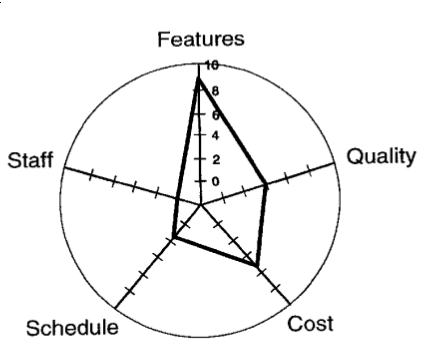
\includegraphics[width=\linewidth]{images/17_ej1_infoInterno.png}
  \caption{Sistema de información interno}
\endminipage\hfill
\minipage{0.32\textwidth}
  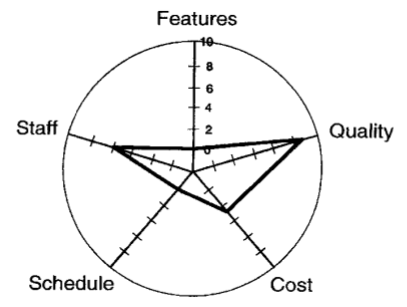
\includegraphics[width=\linewidth]{images/17_ej2_appComercial.png}
  \caption{Aplicación comercial competitiva}
\endminipage\hfill
\minipage{0.32\textwidth}%
  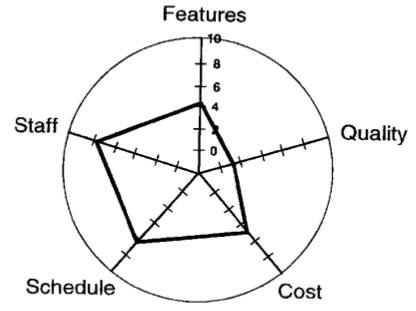
\includegraphics[width=\linewidth]{images/17_ej3_qualityDriven.png}
  \caption{``Quality Driven''}
\endminipage
\end{figure}

\subsubsection{Identificación preliminar de requerimientos}
Otra de las tareas de un gerente es la identificación preliminar de requerimientos. Es un paso necesario para hacer la planificación, dado que inicialmente se usan para la estimación. Este paso involucra no solo requerimientos funcionales, sino también \textbf{atributos de calidad}.


\subsubsection{Otros}
Otras tareas importantes a realizar antes de comenzar un proyecto involucran:
\begin{itemize}
	\item Elección de un modelo de ciclo de vida.
	\item Definición de un proceso para el proyecto.
	\item Definición de relación gente / duración y curva de \emph{staffing} (cuidado con el ``mito hombre hora''\footnote{El \textbf{mito hora hombre} afirma que es falso que las horas y los hombres son intercambiables. \emph{Por muchas mujeres que ponga a la tarea, no voy a tener un bebé en menos de 9 meses}.} y la ``zona imposible''\footnote{La \textbf{zona imposible} es el momento en el cual, por más que agregue más gente, no puedo comprimir más el tiempo del proyecto.}).
\end{itemize}

\subsection{WBS}
Un (\texttt{WBS}) (\emph{Work Breakdown Structure}) es un gráfico que muestra la división de un proyecto o el producto en partes más pequeñas y manejables, hasta el nivel en que será ejecutado el control. Es el primer paso del armado de un cronograma.

Para realizar un \texttt{WBS}, es necesario, en primer lugar, definir su propósito (ej: poder estimar o asignar tareas) e identificar el nodo raíz. Luego, se subdivide cada componente en $7\pm2$ subcomponentes hasta que se cumpla con el propósito.

\subsubsection{Tipos de WBS}
Existen tres tipos de \texttt{WBS}:

\subsubsubsection{WBS de proceso}
\begin{itemize}
	\item La raíz identifica el nombre del proyecto.
	\item El segundo nivel identifica elementos mayores - Planificación, organización, análisis de requerimientos, diseño, iteraciones, etc.
	\item Partición de un proceso en subprocesos hasta obtener tareas individuales (1 o 2 personas) a desarrollar en poco tiempo (1 a 2 semanas).
\end{itemize}

\subsubsubsection{WBS de producto}
\begin{itemize}
	\item Altamente relacionado con la arquitectura del producto.
	\item Identifica componentes e interfaces del producto.
	\item Identifica hardware, software y datos.
	\item La raíz identifica el nombre del producto.
	\item Los otros elementos son ítems discretos e identificables de hardware, software y datos.
\end{itemize}


\subsubsubsection{WBS híbrido}
\begin{itemize}
	\item Combina elementos de los dos tipos anteriores.
	\item La raíz es un proceso, alternando elementos de proceso y producto.
	\item La idea es que los procesos producen productos y los subproductos requieren procesos para su desarrollo.
	\item Utilizado por managers que quieren priorizar la estimación y control precisos de cada elemento de producto.
\end{itemize}

\subsubsection{Dependencias}
Para poder optimizar la asignación de recursos es necesario entender las \textbf{dependencias} entre las tareas. Una dependencia es una relación entre dos o más tareas. Esta relación puede ser:
\begin{itemize}
 	\item Fin a comienzo.
 	\item Fin a fin.
 	\item Comienzo a fin.
 	\item Comienzo a comienzo.
 \end{itemize}

A la hora de armar un plan, la fecha de comienzo de tareas debe ser dinámicamente establecida en función de sus dependencias.

\subsubsubsection{Tareas especiales}
Se usa el recurso de \textbf{tarea hito}: es una tarea que tiene duración 0 que tiene un entregable asociado. Se utiliza como punto de control donde confluyen muchas tareas. Suelen tener alguna actividad relacionada.

Además, es necesario considerar e inlcuir \textbf{puntos de revisión y ajuste}, que suelen generar ciclos de tareas.

\subsubsubsection{Dependencias externas}
Es esencial considerar no sólo dependencias entre tareas internas al proyecto sino también dependencias con otros proyectos. Esto involucra no sólo tareas técnicas, sino también de negocios.

Además, no sólo hay que tener en cuenta proyectos ``propios'' sino también proyectos existentes en la organización con impacto en el propio.

Al final se agregan dependencias por contención de recursos: no tiene que ver con la esencia de las tareas, sino con que no tengo gente para hacer todas esas tareas en paralelo.


\subsubsection{Camino crítico}
Un \textbf{camino crítico} en un \texttt{WBS} es una secuencia de tareas en el \texttt{DAG} del proyecto cuyo atraso provoca atrasos en el fin del proyecto.

Toda camino tiene asociado un \emph{\textbf{slack}} (margen): una cantidad de tiempo que se puede atrasar esa rama sin que se atrase todo el proyecto. Un camino es crítico si su \emph{slack} es 0.

\ig{0.3}{18_wbsDag.png}

~\newline

Es importante tener en cuenta los caminos críticos porque, lógicamente, es donde debe ir el mayor esfuerzo, más recursos, más atención, etc. Es lo que tengo que acortar si quiero acortar todo el proyecto. Además es crucial en la estimación: un análisis del plan para comprimir cronogramas debe comenzar por las tareas críticas.

El \emph{\textbf{lag}} es el atributo de una arista que determina el tiempo mínimo que tiene que pasar entre que termino una tarea y puedo empezar la siguiente.


\subsubsection{Diagrama de Gantt}
Un \textbf{diagrama de Gantt} es un gráfico que me muestra el ordenamiento de las tareas a lo largo del tiempo. Muestra tareas con responsables, fechas, secuencia de ejecución y costos directos. Sirve fundamentalmente como referencia para la ejecución y control del proyecto. Para presentaciones se suelen usar sólo diagramas de hitos o de componentes de alto nivel, sin incluir la descripción detallada de actividades.

\ig{0.4}{19_gant.png}

\subsubsection{Otras definiciones}
\begin{itemize}
	\item \textbf{Línea de base}: Es una versión estable de mi plan que se usa como base para hacer el seguimiento. Es contra lo que voy a comparar la planificación actual.
	\item \textbf{Programación por valor acumulado}: tiene que ver con la medición del progreso. Para medir avance se usa la fórmula de valor acumulado: definición de pesos a los entregables de los hitos, para medir avance (no esfuerzo). Informalmente, se asocian entregables a cada hito. Esos esos entregables tienen un peso que voy acumulando a medida que voy logrando.
\end{itemize}

\subsection{Gestión de riesgos}
En el contexto de gestión de proyectos, se define un \textbf{riesgo} como un problema que todavía no ocurrió. Un \textbf{problema} es un riesgo que se manifestó.

Los riesgos tratan sobre posibles eventos en el futuro y están caracterizados por:
\begin{itemize}
	\item \textbf{Probabilidad} de que el riesgo se manifieste.
	\item \textbf{Impacto} si lo hace.
\end{itemize}

Se define la \textbf{exposición} a un riesgo como $probabilidad\ \times\ impacto$. Uno de los principales problemas de la ingeniería del software es que no hay forma exacta de cuantificar estas medidas. Se suelen trabajar ``artesanalmente''.

Estas dos caracterizaciones definen las dos principales formas de atacar un riesgo: reducir la probabilidad de que ocurra o su impacto negativo si ocurre.

Una \textbf{fuente de riesgo} es algo que me indica que un riesgo está presente.

\subsubsection{Sistematización}
Para sistematizar el tratamiento de riesgos, la \texttt{IEEE} propone realizar ciclos de:
\begin{itemize}
	\item Identificación de riesgo.
	\item Análisis de riesgo.
	\item Planificación.
	\item Seguimiento del plan.
	\item Aplicación de medidas de control.
\end{itemize}

\ig{0.5}{20_sistematizacionRiesgos.png}


\subsubsection{Identificación de riesgos}
Existen numerosos métodos para identificar riesgos:

\begin{itemize}
	\item Brainstorms.
	\item Reporte periódico de riesgos.
	\item Cuestionario de identificación taxonómica. Es un cuestionario de 194 preguntas si/no. Es obsoleto.
	\item Reportes voluntarios de riesgos.
	\item Listas de riesgos comunes,
\end{itemize}


\subsubsection{Documentación}
Dado que los riesgos son algo inevitable e inherente del desarrollo de software, es importante que queden bien documentados. Para esto se recomienda usar la representación de Gluch:

\begin{center}
	``\textbf{Dado que} [condiciones], \textbf{entonces, posiblemente, } [consecuencias]''
\end{center}

~\newline

Para categorizar los riesgos se los ordena en una matriz de probabilidad $\times$ impacto llamada \textbf{matriz de magnitudes}:

\ig{0.4}{21_categoriaRiesgo.png}


Otro aspecto de la documentación involucra la definición de prioridades. Una vez categorizados los riesgos en la matriz de magnitudes, ordenamos los riesgos según la matriz de magnitudes, ignorando los riesgos de baja magnitud. Para los riesgos de igual magnitud ponemos primero los que requieran acciones correctivas con más urgencia y/o impacto.

Siempre tratamos de quedarnos con los 5 o 10 riesgos con mayor exposición.

\subsubsection{Planificación}
Un \textbf{plan de contingencia} es el conjunto de medidas que han de tomarse si un riesgo se manifiesta. Es muy importante que los planes de contingencia estén bien documentados incluyendo, entre otros en qué circunstancias y quién aplica el plan de contingencia. Además, debe ser implementable.


\subsection{Plan de gestión de proyecto}
Armar un plan de proyecto es más complejo que simplemente armar un cronograma. Incluye cosas como:
\begin{itemize}
	\item Organización del proyecto.
	\item Definición de la estructura interna.
	\item Modelo de ciclo de vida
	\item Infraestructura.
	\item Roles y responsabiliaddes.
	\item Gestión de configuración.
	\item QA.
	\item Gestión de calidad.
	\item Comienzo del proyecto.
	\item Plan de trabajo / cronograma.
	\item Plan de control.
	\item Gestión de riesgos.
	\item Cierre del proyecto.
	\item Organización de planes de proceso.
\end{itemize}

El \textbf{plan de gestión de proyecto} es un documento consistente y coherente para guiar la ejecución y el control del proyecto. Su uso está reglamentado en un estándar de la \texttt{IEEE}.


\newpage

\section{Atributos de calidad}
La \textbf{ingeniería de requerimientos} es una forma disciplinada y sistemática de llegar desde las necesidades de los usuarios hasta una especificación. Para definir correctamente una arquitectura, es imprescindible conocer tres elementos del software:
\begin{itemize}
	\item Funcionalidad ``de negocio'' (requerimientos funcionales).
	\item Atributos de calidad (requerimientos no-funcionales).
	\item Restricciones.
\end{itemize}

Un proyecto de software no se compone enteramente de su funcionalidad \textbf{de negocio}. También existen los \textbf{atributos de calidad} (``ilities''), que referencian características específicas que debe tener el sistema. Antiguamente se llamaban requerimientos no-funcionales. Existen numerosos atributos de calidad, los tratados en la materia son:

\begin{itemize}
	\item Performance.
	\item Disponibilidad.
	\item Testeabiliad.
	\item Modificabilidad.
	\item Usabilidad
	\item Seguridad.
\end{itemize}

(\emph{Sugerencia: un acrónimo para recordarlos es \textbf{PeDiTe MoUsSe}.})

Es importante notar que estos problemas no son completamente independientes, sino que se afecan mucho entre si. Es común que una medida que se tome para mejorar uno de estos atributos de estos de calidad vaya en detrimento de otra. Por ejemlo, una mejora en seguridad suele empeorar la usabilidad de un sistema.

Según la \texttt{IEEE}, la \textbf{calidad} ``\emph{La calidad de un software es el grado en el que un software tiene una combinación deseada de atributos}''.

~\newline
Para atacar los atributos de calidad, se usan \textbf{tácticas} de arquitectura (ver \ref{tacticas}). Estos no son objetivos en si mismos, sino formas de alcanzar atributos de calidad.

\subsection{Generales vs Concretos}
\partir{0.5}{0.5}{\underline{Generales:}
\begin{itemize}
    \item Son independientes de un sistema específico y por lo tanto pueden, potencialmente, pertenecer a cualquier sistema.
    \item Son una guía para saber qué preguntar o pensar en escenarios candidatos.
    \item Están ordenados por atributo de calidad.
\end{itemize}
}{\underline{Concretos}
\begin{itemize}
    \item Son específicos a un sistema, instanciando cada uno de sus atributos.
\end{itemize}}


\subsection{Los 6 atributos}
\subsubsection{Disponibilidad}
El atributo de calidad de \textbf{disponibilidad} está relacionado con las fallas (\emph{failures}) que puede tener el sistema y sus consecuencias asociadas. Se considera que ocurre una \textbf{falla} (\emph{failure}) un sistema no entrega más un servicio de acuerdo con su especificación. Estas fallas (\emph{failures}) son observables por los usuarios.

La disponibilidad es la probabilidad de que un sistema esté disponible cuando se lo necesite. Un sistema se dice \textbf{tolerante a fallas} si puede seguir operando en presencia de fallas.

Es importante entender la distinción entre los siguientes conceptos:
\begin{itemize}
	\item \emph{\textbf{Fault}}: un paso, proceso o definción incorrecta en un sistema que causa que el programa no responda en la forma esperada. Es una debilidad inherente al proceso de desarrollo de software que redunda en un \emph{failure}.
	\item \emph{\textbf{Failure}}: la incapacidad de un sistema o componente de realizar sus funciones requeridas por su especificación.
	\item \emph{\textbf{Error}}: una diferencia entre el valor observado o medido por un cómputo y el valor ``correcto'', especificado por la teoría.
\end{itemize}

Se define el \textbf{tiempo de reparación} como el tiempo hasta que la falla no es más observable.

\subsubsubsection{Tipos de fallas}
\begin{itemize}
    \item Crash faliure: el sistema funciona perfectamente hasta que ocurre un error inesperado.
    \item Omission faliure: el sistema falla recibiendo requerimientos, enviando o recibiendo mensajes.
    \item Timing faliure: el sistema responde fuera de los tiempos esperados.
    \item Response faliure: respuesta del sistema incorrecta o se desvía del flujo de control correcto.
\end{itemize}

\subsubsubsection{Medidas para hacer un sistema más tolerante a fallas}
\begin{itemize}
    \item \emph{Voters}: un ``voter'' recibe entradas y replica en la salida el valor que tenga la mayoría de sus entradas.
    \item Redundancia de voters.
    \item Sistemas duplex: poner $2n+1$ procesadores que computen lo mismo y voten.
\end{itemize}






















\subsubsubsection{Ejemplo}
\begin{itemize}
	\item ``En zonas donde la cobertura 3G sea débil o inexistente, se debe mantener la conexión entre las Terminales de Cobro móviles y el Sistema Central utilizando paquetes GSM SMS''.
	\item ``Si la comunicación entre las terminales de cobro y el Sistema Central se pierde, o los tiempos de transmisión son prohibitivos, las terminales de cobro deben seguir funcionando en modo offline, de forma transparente al usuario''.
\end{itemize}

\subsubsection{Modificabilidad}
El atributo de \textbf{modificabilidad} hace referencia al costo de realizar cambios en el sistema. Este costo no sólo referencia el costo económico de los cambios, sino también tiempo y esfuerzo invertido.

Estos cambios pueden ser:
\begin{itemize}
	\item Funcionalidad.
	\item Plataforma.
	\item Otros atributos de calidad.
	\item Interfaces.
\end{itemize}

Hace un cambio involucra:
\begin{itemize}
	\item Especificarlo.
	\item Diseñarlo.
	\item Implementarlo.
	\item Probarlo.
	\item Ponerlo en producción.
\end{itemize}


\subsubsubsection{Ejemplo}
\begin{itemize}
	\item ``Si bien existen varias maneras para realizar la recarga de una tarjeta de proximidad, es probable que en el futuro se desee aceptar nuevas formas de pago, por ejemplo, vía web. Es por ello que se requiere tener un sistema fácil de extender a nuevas formas de pago sin que esto impacte demasiado y sea rápido de implementar''.
	\item ``Se pretende, en un futuro, implementar un sistema tarifario basado en zonas, en el cual el costo del pasaje este en relación con la cantidad de zonas que el pasajero atraviesa y no respecto de la cantidad de transportes que utilice. Por lo tanto, se espera que el sistema sea fácil de modificar para aceptar nuevas formas de realizar el cobro de los pasajes''.
\end{itemize}

\subsubsection{Performance}
El atributo de \textbf{performance} está relacionado con el tiempo que le lleva al sistema responder a un evento (interrupción, mensaje, pedido, etc) que ocurre. Es extremandamente difícil de expresar porque depende de innumerables factores, tales como:
\begin{itemize}
 	\item \textbf{Latencia}: tiempo entre la llegada del estímulo y el inicio de la respuesta del sistema.
	\item \textbf{Jitter}: variación en la latencia.
	\item \textbf{Deadlines}: límites de tiempo para un proceso.
	\item \textbf{Throughput}: cantidad de transacciones que el sistema puede procesar en un período de tiempo.
	\item Eventos no procesados.
\end{itemize}

\subsubsubsection{Ejemplo}
\begin{itemize}
	\item ``Se requiere que el sistema sea capaz de realizar las operaciones de autenticación y cobro en a lo sumo 1 segundo ya que, de otro modo, no sería bien recibido los usuarios, ni los choferes de colectivos. Esto es especialmente crítico en horas pico''.
\end{itemize}

\subsubsection{Seguridad}
El atributo de \textbf{seguridad} predica sobre la habilidad de un sistema para resistir usos no autorizados y seguir proveyendo sus servicios a usuarios legítimos. Involucra:

\begin{itemize}
	\item \textbf{Confidencialidad}: se garantiza que la información sea accesible sólo por aquellas personas autorizadas.
	\item \textbf{Integridad}: se salvaguarda la exactitud y totalidad de la información y los métodos de procesamiento. La integridad incluye: la integridad de los datos (el contenido) y el origen de los mismos.
	\begin{itemize}
		\item Integridad de datos: nadie altere el contenido.
		\item Integridad de origen (\emph{nonrepudiation}): el origen de los datos sea cierto.
	\end{itemize}
	\item \textbf{Disponibilidad}: se garantiza que los usuarios autorizados tengan acceso a la información y a los recursos relacionados con la misma, toda vez que lo requieran.
\end{itemize}

Se considera parte de integridad la \textbf{auditabilidad}, que habla de la habilidad de un sistema para hacer un seguimiento de actividades realizadas.

\subsubsubsection{Ejemplo}
\begin{itemize}
	\item ``Es crítico que nadie fuera del Sistema Central y el Banco Nación conozca ninguno de los datos de los usuarios, sus compras realizas, recargas efectuadas, etc''.
	\item ``Es también muy importante que los datos (por ej. de una recarga) lleguen de forma correcta, y sin ningún tipo de modificación por factores externos como la forma de transmisión''.
	\item ``Deben de detectarse potenciales diferencias malintencionadas entre los saldos almacenados de forma local en las tarjetas y los valores guardados para las mismas en el Sistema Central. Nadie debería viajar gratis''.
	\item ``El Sistema Central debe mantener un registro completo de absolutamente todos los viajes que se realizaron''.
\end{itemize}

\subsubsection{Usabilidad}
La \textbf{usabilidad} está relacionada con la facilidad con la cual un usuario puede cumplir una tarea o utilizar un servicio ofrecido por el sistema y el tipo de soporte que provee el sistema.

Involucra cosas como:
\begin{itemize}
	\item Aprender la funcionalidad del sistema.
	\item Usar el sistema eficientemente.
	\item Minimizar el impacto de los errores.
	\item Adaptar el sistema a las necesidades de los usuarios.
	\item Aumentar confianza y satisfacción.
\end{itemize}

\subsubsubsection{Testeabiliad}
\begin{itemize}
	\item ``Dado que en los colectivos será el propio pasajero quien determine el valor del pasaje mediante una interfaz de tipo touchscreen, se desea que la misma sea intuitiva y permita realizar dicha operación de manera rápida y sencilla en la mayoría de los casos''.
	\item ``Se quiere que el sistema de información de tarifas, rutas, y tiempos sea accesible para personas con discapacidades visuales''.
\end{itemize}


\subsubsection{Testeabiliad}
La \textbf{testeabilidad} es la posibilidad de ver el \emph{estado interno} de la aplicación.


\subsection{Especificación}
Uno de los principales problemas de los atributos de calidad es que suelen estar pobremente o nulamente especificados. No se suelen analizar sus dependencias, ni se les da importancia a la hora de hacer una especificación formal. Sin embargo, su nivel de importancia puede llegar a ser muy alto (varía dependiendo del proyecto particular).

Una forma de especificar un atributo de calidad es mediante un \texttt{QAS} (\textbf{\emph{Quality Attribute Scenario}}). Una \texttt{QAS} es una tupla:
\begin{itemize}
	\item \textbf{Fuente}: interna o externa.
	\item \textbf{Estímulo}: condición que debe ser tenida en cuenta al llegar al sistema Entorno: condiciones en las cuales ocurre el estímulo.
	\item \textbf{Artifact}: el sistema o partes de él afectadas por el estímulo
	\item \textbf{Response}: qué hace el sistema ante la llegada del estímulo.
	\item \textbf{Resonse measure}: cuantificación de un atributo de la respuesta.
\end{itemize}

\subsubsection{Ejemplos}
\subsubsection{Disponibilidad}
``Si la comunicación entre una Terminal de Cobro móvil y el Sistema Central se pierde, o los tiempos de transmisión son prohibitivos, la Terminales de Cobro debe de seguir funcionando en modo offline, de forma transparente al usuario''.

\begin{itemize}
	\item Fuente: Interno al sistema.
	\item Estímulo: Tiempo promedio transacciones mayor a 1 seg.
	\item Entorno: Operación normal.
	\item Artefacto: Terminal de Cobro.
	\item Respuesta: La terminal pasa a modo offline, utilizando la información local almacenada en las tarjetas y logueando toda operación realizada para que este lista cuando la conexión se restablezca.
	\item Medición: No se requieren acciones adicionales por parte del usuario, y no se ve afectada la performance ($\leq$ 1 seg. por trans.).
\end{itemize}


\subsubsection{Modificabilidad}
``Se pretende, en un futuro, implementar un sistema tarifario basado en zonas, en el cual el costo del pasaje este en relación con la cantidad de zonas que el pasajero atraviesa y no respecto de la cantidad de transportes que utilice. Por lo tanto, se espera que el sistema sea fácil de modificar para aceptar nuevas formas de realizar el cobro de los pasajes''.

\begin{itemize}
	\item Fuente: Ministerio de Planificación.
	\item Estímulo: Agregar al sistema la división por zonas y basar el costo de los pasajes en las mismas.
	\item Entorno: En tiempo de diseño.
	\item Artefacto: Sistema.
	\item Respuesta: Cambio efectuado sin efectos secundarios, el pago se efectúa con la nueva modalidad de cobro.
	\item Medición de la respuesta: Se invierten menos de 550 horas hombre. La usabilidad no se ve afectada negativamente.
\end{itemize}


\subsubsection{Performance}
``Se requiere que el sistema sea capaz de realizar las operaciones de autenticación y cobro en a lo sumo 1 segundo ya que, de otro modo, no sería bien recibido por los usuarios, ni los choferes de colectivos. Esto es especialmente crítico en horas pico''.
\begin{itemize}
	\item Fuente: Pasajero.
	\item Estímulo: Se aproxima o inserta una tarjeta para realizar el pago de un pasaje.
	\item Entorno: En operación normal y hora pico.
	\item Artefacto: Terminal de cobro.
	\item Respuesta: Se concreta la operación de la venta del pasaje.
	\item Medición de la respuesta: tiempo de respuesta total $\leq$ 1 seg.
\end{itemize}

\subsubsection{Seguridad}
``Es crítico que nadie fuera del Sistema Central y el Banco Nación conozca ninguno de los datos de los usuarios, sus compras realizas, recargas efectuadas, etc''
\begin{itemize}
	\item Fuente: Atacante externo.
	\item Estímulo: Captura un mensaje encriptado e intenta vulnerar la seguridad para obtener información confidencial de las transacciones de los usuarios.
	\item Entorno: Operación Normal.
	\item Artefacto: Módulos de encriptación de las terminales y el Sistema Central.
	\item Respuesta: Los datos no son accesibles al usuario en tiempos razonables (miles de años).
	\item Medición de la respuesta: (tiempo para ``romper'' el sistema, \% de casos en los que el ataque no es exitoso).
\end{itemize}

\subsubsection{Usabilidad}
``Dado que en los colectivos será el propio pasajero quien determine el valor del pasaje mediante una interfaz de tipo touchscreen, se desea que la misma sea intuitiva y permita realizar dicha operación de manera rápida y sencilla en la mayoría de los casos''.

\begin{itemize}
	\item Fuente: Pasajero.
	\item Estímulo: Selecciona pasaje que quiere adquirir.
	\item Entorno: Operación normal.
	\item Artefacto: Terminal de Cobro/Recarga, Interfaz gráfica.
	\item Respuesta: El pasajero realiza la operación satisfactoriamente.
	\item Medición de la respuesta: En test usabilidad, 95\% de los pasajeros pueden realizar la operación, sin ningún tipo de ayuda de otra persona, la primera vez que se enfrentan al sistema, y en menos de 20 segundos.
\end{itemize}


\subsection{Quality Attribute Workshops}
Un \emph{\textbf{Quality Attribute Workshop}} (\texttt{QAW}) es un método que relaciona los \emph{stakeholders} de un sistema de manera temprana en el ciclo de vida para descubrir los atributos de calidad clave en un sistema de software.

Sus pasos son:

\begin{itemize}
	\item Presentación del método: describir el propósito del \texttt{QAW} y a los ``stakeholders'' (posición en la organización y rol en el sistema)
	\item Presentación del negocio / misión: presentación realizada por un representante de los stakeholdes cuyo objetivo principal es entender la motivación para construir el sistema.
	\item Presentación del plan de arquitectura: un representante técnico presenta lo que se sepa sobre la arquitectura:
	\begin{itemize}
		\item Planes y estrategias.
		\item Requerimientos y restricciones clave.
		\item Diagramas de alto nivel.
	\end{itemize}
	\item Identificar drivers arquitectónicos: primera depuración de los resultados de los pasos anteriores. Involucra una clasificación en requerimientos, restricciones y atributos de calidad requeridos.
	\item Brainstorming de escenarios: consiste en buscar escenarios de los 3 tipos (caso de uso, crecimiento, exploratorios) y se los documenta como estímulo, entorno o respuesta.
	\item Consolidación de escenarios: los facilitadores agrupan escenarios similares
	\item Definición de prioridades de escenarios: cada stakeholders ``vota'' por hasta un 30\% de los escenarios consolidados.
	\item Refinamiento de escenario: se refinan los 4 o 5 escenarios más votados.
\end{itemize}


\section{UML}
Hacia principios de los '90, coexistían distintas notaciones y enfoques para modelado de objetos. En ese contexto, \texttt{UML} (\emph{Unified Modeling Language}) surgió como un estándar de modelado que combina modelos nuevos y existentes, e intenta cubrir todas las necesidades de especificación de un sistema de software.

\texttt{UML} \textbf{no es una metodología ni un proceso, es una notación estándar de modelado para capturar el conocimiento semántico de un problema y su solución}.

Un \textbf{proceso} es una descripción de actividades que deben realizarse en un determinado orden (en este caso para crear o modificar un sistema de software). Describe qué hacer, cómo hacerlo, cuándo hacerlo, qué roles deben hacerlo y el motivo por el que se hace. Debe ser: reproducible, definido, medible y mejorable.


\section{Unified Process}
El \textbf{unified process} es un marco de desarrollo de software que se caracteriza por estar dirigido por casos de uso, centrado en la arquitectura y por ser iterativo e incremental. Se centra en la \textbf{arquitectura}, pero está dirigido por casos de uso.

Es importante notar que \texttt{UP} es un \emph{framework}: se puede (y debe) adaptar a las características de un proyecto.

Se define el concepto de \textbf{\emph{risk-based development}}: los riesgos guían la elección de la funcionalidad.

\subsubsection{Buenas prácticas}
\begin{itemize}
	\item Desarrollar iterativamente.
	\item Administrar los requerimientos.
	\item Usar arquitecturas de componentes.
	\item Modelar visualmente (UML)
	\item Verificar la calidad.
	\item Controlar los cambios.
\end{itemize}


\subsection{Iteraciones}
A diferencia de scrum, en \texttt{UP} el resultado de cada iteración es un sistema funcionando, aunque no necesariamente ``potentially shippable''. Hay que tenter cuidado con las ``salidas a producción intermedias''.

Sin embargo, al igual que en scrum, hay aprendizaje entre las itearciones y se aplica el concepto de \emph{timed boxing} (entre 2 y 12 semanas). Además se busca el feedback del usuario.

Las iteraciones no son estrictamente secuenciales. Las disciplinas se superponen.

\subsubsection{Fases}

$\left.\begin{minipage}{11cm}
\begin{itemize}
	\item Inicio del proyecto: definir contexto, factibilidad y objetivos.
	\item Elaboración: funcionalidad (alcance) y arquitectura básica.
\end{itemize}
\end{minipage}\right\rbrace$
\begin{minipage}{10cm}
Etapa de Ingeniería.
\end{minipage}

~\newline\vspace{-0.2cm}

$\left.\begin{minipage}{11cm}
\begin{itemize}
	\item Construcción: desarrollar el producto iterativamente.
	\item Transición: liberar el producto para uso real.
\end{itemize}
\end{minipage}\right\rbrace$
\begin{minipage}{10cm}
Etapa de Producción.
\end{minipage}


\subsubsection{Hitos}
En \texttt{UP}, un \textbf{hito} es un punto de control para revisar el avance del proyecto. Tienen entregables asociados para evaluación.

Existen dos tipos de hitos:
\begin{itemize}
	\item Principales al finalizar una fase (visión, arquitectura básica, capacidad inicial, producto final).
	\item Secundarios al finalizar una iteración.
\end{itemize}

Algunas definiciones:
\begin{itemize}
	\item \textbf{Disciplinas}: organizan las actividades del proyecto. Cada disciplina de desarrollo genera modelos de UML (casos de uso, análisis, diseño, deployment, etc).
	\begin{itemize}
		\item De desarrollo: requerimientos, análisis, arquitectura, diseño, implementación, pruebas, deployment.
		\item De gestión: administración de riesgos, planificación y seguimiento, SCM (software configuration management), etc.
	\end{itemize}
	\item \textbf{Artefactos}: Cualquier tipo de información generada por el equipo de desarrollo
\end{itemize}

En general el número de artefactos generados es muy grande. Luego, es preciso definir cuáles se harán en un desarrollo concreto:
\begin{itemize}
	\item
\end{itemize}


\subsubsection{Fase de incepción}
Los propósitos de la fase de incepción son:
\begin{itemize}
 	\item Establecer el ``caso de negocio'' para un sistema nuevo o mejoras a uno existente.
 	\item Además se debe especificar el alcance del proyecto.
 \end{itemize}

Lo que se espera obtener de la fase de incepción es:
\begin{itemize}
	\item Visión de los requerimientos (10-20\%).
	\item Caso de negocio.
	\begin{itemize}
		\item Criterios de éxito.
		\item Estimación de recursos requeridos.
		\item Evaluación inicial de riesgos.
	\end{itemize}
\end{itemize}
Su hito principal es: ``Lifecycle objectives''.

\subsubsection{Fase de elaboración}
Los propósitos de la fase de elaboración son:
\begin{itemize}
	\item Analizar el dominio del problema.
	\item Establecer una base sólida de arquitectura.
	\item Atacar principales riesgos.
	\item Desarrolloar un plan completo.
\end{itemize}


Lo que se espera obtener de la fase de elaboración es:
\begin{itemize}
	\item Modelo de dominio y casos de uso (80\% completo).
	\item Arquitectura probada y documentada.
	\item Tener revisado el caso de negocio.
	\item Tener terminado el plan de desarrollo.
\end{itemize}


\subsubsection{Fase de construcción}
En construcción se especifica, desarrolla y prueba el producto de manera incremental.

\subsubsection{Fase de transición}
En transición se llevan a cabo todas las tareas necesarias para una salida a producción:
\begin{itemize}
	\item Instalación.
	\item Configuración.
	\item Entrenamiento.
	\item Soporte.
	\item Mantenimiento.
\end{itemize}

No se deben confundir las iteraciones de transición con los ciclos de pruebas.

\subsection{Ventajas y desventajas}
\partir{0.5}{0.5}{\underline{Ventajas:}
\begin{itemize}
	\item Buenas Prácticas
	\item Casos de uso
	\item Iteraciones
	\item Arquitectura
	\item \texttt{UML}
\end{itemize}
}{\underline{Problemas:}
\begin{itemize}
	\item ``Sopa de prácticas''
	\item Demasiado grande
	\item Adopción muy difícil
	\item ``Nobody reads process books''
	\item Extensión difícil
	\item \emph{Process gap}.
\end{itemize}}

\section{Arquitecturas}
La \textbf{arquitectura de un sistema de software} define el sistema en términos de elementos e interacción entre ellos. Es como una descripción de ``alto nivel'' del diseño. Muestra correspondencia entre requerimientos y elementos del sistema construido.

Resuelve atributos de calidad en el nivel del sistema, como escalabilidad, flexibilidad, confiabilidad y performance

Informalmente, intenta plantear una respuesta al problema de construir un puente entre los requerimientos y las soluciones (diseño detallado / implementación).

Las arquitecturas son importantes porque son un paso clave para poder lograr el reuso a gran escala y ayudar a que la ingeniería de software empiece a asemejarse a otras disciplinas de la ingeniería. Además, faculuta la comunicación temprana entre ``stakeholders'' y ayuda a tomar decisiones tempranas de diseño tales como:
\begin{itemize}
	\item Define restricciones de implementación
	\item Afecta la estructura organizativa
	\item Posibilita o inhibe atributos de calidad de un sistema
	\item Facilita el razonamiento sobre cambios y su implementación
	\item Permite estimaciones más precisas
\end{itemize}

Además, la arquitectura hace posible la abstracción transferible de un sistema: los sistemas pueden ser construidos a partir de elementos externos, lo que permite el ``desarrollo basado en templates''.

\subsection{Definiciones}
\textbf{Según Bass y Clemens, la arquitectura de software de un sistema de computación es el conjunto de estructuras necesarias para razonar sobre el sistema. Comprende elementos de software, relaciones entre ellos y propiedades entre ambos}.

Un \textbf{estilo} (o patrón arquitectónico) es una descripción de tipos de relaciones y elementos, junto con restricciones sobre cómo deben usarse (ej. ``client server'').

Una \textbf{arquitectura de referencia} es una división común de funcionalidad mapeada a elementos que cooperativamente implementan esa funcionalidad y flujos de datos entre ellos. Ej: uso de sensores y actuadores en aplicaciones de robótica.

Una arquitectura es \textbf{heterogénea} si resulta de la combinación de distintos estilos arquitectónicos.

\subsection{Los tres principios fundamentales}
\begin{itemize}
	\item Toda aplicación tiene una arquitectura.
	\item Cada aplicación tiene al menos un arquitecto.
	\item La ``arquitectura'' \textbf{no} es una fase del desarrollo.
\end{itemize}


\subsection{¿Qué hace que una arquitectura sea buena?}
\begin{itemize}
	\item Producto de un único arquitecto o un pequeño grupo de arquitectos con un claro líder. \textbf{Integridad conceptual}.
	\item El equipo de arquitectura debe contar con requerimientos funcionales y atributos de calidad requeridos que sean claros.
	\item La arquitectura debe estar documentada.
	\item La arquitectura debe ser revisada por los \emph{stakeholders}.
	\item Debe ser evaluada cuantitativamente antes de que sea tarde.
	\item Debe permitir una implementación incremental.
	\item Módulos bien definidos basados en el ocultamiento de la información.
	\item Interfaces claramente definidas.
	\item No dependiente de un único producto comercial.
	\item Usa un grupo pequeño y claro de patrones de interacción.
\end{itemize}


\subsection{Documentación de una arquitectura}
Elementos esenciales:
\begin{itemize}
    \item Descripción de los requerimientos: contexto del negocio, “rationale” para el producto, dominio.
    \item Descripción del contexto: sistemas con quienes interactúa, interfaces externas.
    \item Uso de diagramas de arquitectura: con prosa y descripción de cajas y líneas.
    \item Consideración de restricciones de implementación (en la medida en que impactan la arquitectura).
    \item Explicación del diseño arquitectónico: como ataca los requerimientos y las restricciones de diseño. Alternativas.
\end{itemize}

Hay varios puntos clave a tener en cuenta para documentar una arquitectura:
\begin{itemize}
    \item El documento está escrito para el lector, no quien lo escribe.
    \item Evitar ambigüedad.
    \begin{itemize}
        \item Explicar la notación – claves.
        \item Adjuntar información adicional, por ejemplo de interfaces.
    \end{itemize}
    \item Usar una organización estándar (qué vistas, template a usar)
    \item Registrar los motivos (explicar el por qué de las decisiones tomadas).
    \item Mantenerla actualizada, pero no demasiado.
    \item Revisarla.
\end{itemize}

\subsection{Arquitectura vs diseño}
No hay consenso con respecto a la relación entre arquitectura y diseño. La visión más aceptada es que la arquitectura es una parte del diseño, que también involucra decisiones no arquitectónicas (que pueden convertirse en arquitectónicas más adelante, dependiendo de la visibilidad de sus módulos).

Recordemos que la definición de \textbf{diseño} es: ``formar un plan o esquema en la mente para ejecución posterior''.

\subsection{ADD}
\texttt{ADD} (\emph{Attribute Driven Design}) es un método para desarrollar una arquitectura que consiste en:
\begin{itemize}
    \item Elegir el módulo a descomponer.
    \item Refinar el módulo:
    \begin{itemize}
        \item Elegir drivers de arquitectura a partir de Escenarios de Atributos de Calidad y requerimientos funcionales.
        \item Elegir un patrón arquitectónico que satisfaga los drivers.
        \item Instanciar módulos y asignar funcionalidad / representar usando vistas.
        \item Definir interfaces de módulos hijos.
        \item Verificar y refinar casos de uso y escenarios.
    \end{itemize}
    \item Iterar.
\end{itemize}



\section{Estilos arquitectónicos}
Un \textbf{estilo arquitectónico} es una colección de decisiones de arquitecturas que son aplicables en un contexto de desarrollo, se encuentran repetidamente en la práctica y tiene propiedades beneficiosas que permiten y justifican su reuso. Informalmente, es una descripción (de muy alto nivel y sin hablar de funcionalidad específica) de tipos de relaciones y elementos, junto con restricciones sobre cómo deben usarse.

Son el equivalente a los patrones de diseño, pero con ciertas diferencias. Los estilos arquitectónicos tienen en común con los patrones que ambos proveen un ``lenguaje común'' y una abstracción con la que se describen clases de sistemas. La principal diferencia es que un patrón es una solución a un problema recurrente, mientras que un estilo es más general y no requiere de un problema para su aparición.


Los estilos arquitectónicos tienen restricciones topológicas que determinan cómo se puede hacer la composición de los elementos que involucran (por ejemplo, ``los elementos de un \emph{layer} sólo se pueden comunicar con los de un \emph{layer} inferior'') y provee semántica para esos elementos.

Es importante notar que un estilo arquitectónico \textbf{no define la funcionalidad de un sistema}. Es abstracto.

\subsection{Ventajas}
\begin{itemize}
	\item Reuso de diseños: soluciones maduras aplicadas a problemas nuevos.
	\item Reuso de código: una parte importante del código que implementa la arquitectura puede pasarse de un sistema a otro.
	\item Comunicación.
	\item Portabilidad.
\end{itemize}

\subsection{Taxonomía}
La \textbf{taxonomía} es la ciencia de la clasificación. En este caso, se aplica una clasificación a los estilos arquitectónicos, agrupándolos por características comúnes. No existe una única taxonomía.

Ejemplo:
\ig{0.4}{22_taxonomiaEstilos.png}


\subsection{Estilos}
\subsubsection{Data Flow}
En los estilos tipo \emph{\textbf{data flow}}, la estructura del sistema está basada en transformaciones sucesivas a datos de \emph{input}: los datos entran al sistema y fluyen a través de los componentes hasta su destino final.

Normalmente existe un componente de control que controla la ejecución del resto de los componentes.

Hay dos subestilos:
\subsubsubsection{Batch sequential}
En \emph{\textbf{batch sequential}}, cada paso se ejecuta hasta ser completado, y recién después puede comenzar el siguiente paso. Es usado en aplicaciones clásicas de procesamiento de datos.

\ig{0.4}{23_batchSequential.png}

\subsubsubsection{Pipe and filter}
En \emph{\textbf{pipe and filter}}, cada componente tiene \emph{inputs} y \emph{outputs}. Los componentes leen \emph{streams} de datos de su \emph{input} y producen \emph{streams} de datos en sus \emph{outputs} de forma continua.
\begin{itemize}
    \item \emph{Filters}: ejecutan las transformaciones
    \item \emph{Pipes}: conector
\end{itemize}

\ig{0.5}{24_pipeAndFilter.png}

\subsubsubsection{Ventajas y desventajas}
\partir{0.5}{0.5}{\underline{Ventajas:}
\begin{itemize}
    \item Fácil de entender: la función del sistema es la composición de sus filtros.
    \item Facilidad de extensión – reuso – recambio de filtros.
    \item Posibilidad de ejecución concurrente.
\end{itemize}
}{\underline{Problemas:}
\begin{itemize}
    \item ``Mentalidad batch'', difícil para aplicaciones interactivas.
    \item El orden de los filtros puede ser complejo.
    \item Overhead de parsing y unparsing.
    \item Problemas con tamaño de los buffers.
\end{itemize}}

\subsubsection{Call return}
\textbf{\emph{Call return}} es un estilo arquitectónico orientado a la programación estructurada. Su principal ventaja es su simplicidad y escasa longitud del código. Su desventaja es que su posibilidad de reuso es muy limitada.


~\newline

En contraposición a este estilo, existen arquitecturas orientadas a objetos. Estas arquitectura implementan conceptos como
\begin{itemize}
    \item \emph{Information hiding}.
    \item Encapsulamiento.
    \item Herencia.
    \item Polimorfismo.
\end{itemize}

\partir{0.5}{0.5}{\underline{Ventajas:}
\begin{itemize}
    \item Reuso a gran escala.
    \item Todas las ventajas del encapsulamiento y el \emph{information hiding}.
    \item Correspondencia en los objetos del dominio con objetos del mundo real.
\end{itemize}
}{\underline{Problemas:}
\begin{itemize}
    \item \emph{Information hiding}: las decisiones de diseño que es probable que cambien son ocultadas en un módulo o un conjunto pequeño de módulo.
\end{itemize}}

\subsubsection{Layered}
Las arquitecturas de estilo \textbf{\emph{layered}}, se dividen en \emph{layers} (o capas), cada una de las cuales:
\begin{itemize}
    \item Oculta el nivel siguiente.
    \item Provee servicios al nivel anterior
\end{itemize}

En muchos casos el ``bajar'' de nivel implica acercarse al hardware o software de base. Los niveles van formando ``virtual machines''.

\partir{0.5}{0.5}{\underline{Ventajas:}
\begin{itemize}
    \item Portabilidad.
    \item Facilidad de cambios.
    \item Reuso.
\end{itemize}
}{\underline{Problemas:}
\begin{itemize}
    \item Performace.
    \item La abstracción correcta puede ser difícil de encontrar.
\end{itemize}}


\subsubsection{Client Server}
En las arquitecturas que siguen el estilo \textbf{client server}, los componentes son clientes (que acceden a servicios) o servidores (que proveen servicios). Los servidores no conocen la cantidad o identidad de los clientes, mientras que un cliente si conoce la identidad del servidor a los que se conecta.

\subsubsection{Componentes independientes}
Las arquitecturas de \textbf{componentes componentes} son arquitecturas de procesos que se comunican a través del envío de mensajes. Los componentes son procesos independientes y los conectores representan envío de mensajes, que pueden ser sincrónicos o asincrónicos.

\subsubsubsection{Invocación implícita vs explícita}
\ig{0.4}{25_invocacionImplVsExpl.png}

\subsubsection{Centradas en datos}
Las \textbf{arquitecturas centradas en datos} tienen una estructura de datos central (normalmente una base de datos) y componentes que acceden a ella. Gran parte de la comunicación está dada por esos datos compartidos.

Las hay de dos tipos: \emph{blackboard} y repositorio (cada vez más ocultos en un esquema tipo \emph{layered}).

\subsubsection{Basadas En Eventos}
Las arquitecturas \textbf{basadas en eventos} se organizan como un grupo de componentes independientes con poco acoplamiento
entre sí que permite comunicar a componentes a través de mensajes asincrónicos.

Los componentes disparan la ejecución de otros componentes a través de conectores punto a punto (como \emph{call asincrónico}) o conectores \emph{multi-party}, en los que se envían mensajes a más de un destinatario. Un ejemplo de eso son los \textbf{\emph{publish-subscribe}} en los que algunos componentes se suscriben por medio del conector a un conjunto de eventos proveniente de cualquier publicador y luego otros componentes envían eventos a un conjunto desconocido de receptores (ya suscriptos) a través del conector.

Ejemplo:
\ig{0.4}{26_publishSuscribe.png}


\subsection{Viewtypes}
Un sistema tiene varias estructuras, que pueden dividirse en tres grupos:
\begin{itemize}
    \item De componentes y conectores: aquí los elementos son unidades de \emph{run-time} independientes y los conectores son los mecanismos de comunicación entre esos componentes.
    \item De módulos: los módulos son unidades de implementación, una forma de ver al sistema basada en el código.
    \item Estructuras de asignación (``\emph{allocation}''): Muestra la relación entre elementos de software y los elementos en uno o más entornos externos en los que el software se crea y ejecuta.
\end{itemize}

Llamamos \textbf{viewtypes} a las vistas de arquitecturas orientadas a estas tres estructuras.

\subsubsection{De módulos}
Un \textbf{módulo} es una unidad de código que implementa un conjunto de responsabilidades (una clase, una colección de clases, una capa o cualquier descomposición de la unidad de código. Involucra nombres, responsabilidades, visibilidad de las interfaces, etc). La palabra ``módulo'' hace referencia a una unidad en tiempo de diseño.

Este viewtype involucra las siguientes relaciones:
\begin{itemize}
    \item Descomposición (``es parte de''): los módulos tiene relación del tipo ``es un submódulo de''. Representa la descomposición del código en sistemas, subsistemas, etc
    \item Usos (``depende de''): los módulos tienen relación del tipo ``usa a''. Se dice que un módulo $A$ usa a $B$, si la correcta ejecución de $B$ es necesaria para la correcta ejecución de $A$ (no es lo mismo que invocación). Esta vista hace explícito como una funcionalidad se mapea con una implementación, mostrando la relaciones existentes entre las distintas partes de código que finalmente la implementan.
    \item Clases (``es un''): los módulos en este caso son clases las relaciones son ``hereda de'' u otras asociaciones. Este estilo es útil cuando el arquitecto desea soportar la posible extensión y evolución de la arquitectura. Los módulos son organizados de modo de capturar concordancias y variaciones entre sí. El módulo padre reúne todas las concordancias entre sus hijos, y cada hijo posee las variaciones correspondientes.
\end{itemize}


Se usa \texttt{UML} para graficarlo.

\subsubsubsection{Utilidad}
\begin{itemize}
    \item Construcción:
    \begin{itemize}
        \item Puede proveer un blueprint para el código fuente.
        \item Generalmente es posible establecer mapeos entre módulos y estructuras físicas (como archivos de código fuente).
    \end{itemize}
    \item Análisis:
    \begin{itemize}
        \item Trazabilidad de Requerimientos.
        \item Analiza como los requerimientos funcionales son soportados por las responsabilidades de los distintos módulos.
    \end{itemize}
    \item Análisis de Impacto:
    \begin{itemize}
        \item Permite predecir el efecto de las modificación del sistema.
        \item Comunicación.
        \item Pueden ser utilizadas para explicar las funcionalidades del sistema a alguien no familiarizado con el mismo.
    \end{itemize}
\end{itemize}

\subsubsubsection{Cuando no}
El viewtype de módulos no es de mucha utilidad para la realización de análisis de performance, confiabilidad u otras características asociadas al tiempo de ejecución.

Además, no se ven:
\begin{itemize}
    \item Múltiples instancias de objetos.
    \item Relaciones existentes sólo en tiempo de ejecución.
\end{itemize}




\subsubsubsection{Ejemplo}
Este es un ejemplo de viewtype combinado entre \textbf{módulos} y \textbf{componentes y conectores}.
\ig{0.4}{27_viewtypeModulo.png}

\subsubsection{De componentes y conectores}
Las vistas \textbf{de componentes y conectores} están centradas en procesos que se comunican. Sus elementos son entidades con manifestación \emph{runtime} que consumen recursos de ejecución y contribuyen al comportamiento en ejecución del sistema.

\begin{itemize}
    \item La \textbf{configuración} del sistema es un grafo conformado por la asociación entre componentes y conectores.
    \item Las \textbf{entidades \emph{runtime}} son instancias de tipos de conector o componente.
    \item Los \textbf{componentes} son entidades independientes y sólo se relacionan e interactúan a traves de conectores. La palabra ``conector'' se refiere a unidades en tiempo de ejecución.
    \item Un \textbf{conector} es un componente que representa un camino en la interacción en tiempo de ejecución entre dos o más componentes. El tipo de conector indica la cardinalidad (cantidad de componentes en la interacción), las interfaces que soporta y las propiedades requeridas.
\end{itemize}

Formalmente siempre se asocian puertos de componentes con puertos de conectores (llamados roles): un puerto de componente $p_1$, es vinculado con un rol de conector $r$, si el componente interactúa sobre el conector usando la interfaz descripta por $p_1$ y cumpliendo con la expectativas descritas por $r$.
\ig{0.4}{28_conectores.png}

\subsubsubsection{Ejemplo}
\ig{0.4}{29_ejemploCompoYConect.png}


\subsubsection{De estructuras de asignación}
La vista de \textbf{estructuras de asignación} involucra tres partes:
\begin{itemize}
    \item \textbf{\emph{Deployment}}: muestra cómo el software se asigna a hardware y elementos de comunicación.
    \item \textbf{Implementación}: muestra cómo los elementos de software se mapean a estructuras de archivos en repositorios de control de la configuración o entornos de desarrollo.
    \item \textbf{Asignación de trabajo} : asigna la responsabilidad del desarrollo y la implementación a equipos de programadores.
\end{itemize}

\section{Tácticas} \label{tacticas}
Una \textbf{táctica} busca controlar las respuestas a determinados estímulos. Representa una decisión de diseño. Informalmente, son las cosas que hago durante la etapa de diseño para lograr los atributos de calidad. Se define una \textbf{estrategia} como una colección de tácticas.

\subsection{Relación con los estilos}
Cada estilo puede implementar varias tácticas (Ej: el estilo \emph{layer} implementa la táctica de \emph{information hiding}). Cada una de las tácticas tiene un determinado impacto en los atributos de calidad (Ej: \emph{information hiding} es una táctica para cubrir el atributo de modificabilidad).

\subsection{Tácticas para los atributos}
\subsubsection{Disponibilidad}
\begin{itemize}
    \item \emph{Fault Detection}:
    \begin{itemize}
        \item \emph{Ping / Echo}.
        \item \emph{Heartbeat}.
        \item \emph{Exception}.
    \end{itemize}
    \item \emph{Recovery - Preparation and repair}:
    \begin{itemize}
        \item \emph{Voting}.
        \item \emph{Active redundancy}.
        \item \emph{Passive redundancy}.
        \item \emph{Spare}.
    \end{itemize}
    \item \emph{Recovery - Reintroduction}:
    \begin{itemize}
        \item \emph{Shadow}.
        \item \emph{State resynchronization}.
        \item \emph{Rollback}.
    \end{itemize}
    \item \emph{Prevention}:
    \begin{itemize}
        \item \emph{Removal from service}.
        \item \emph{Transactions}.
        \item \emph{Process monitor}.
    \end{itemize}
\end{itemize}

\subsubsection{Performance}
\begin{itemize}
    \item \emph{Resource Demand}:
    \begin{itemize}
        \item \emph{Increase computation efficiency}.
        \item \emph{Reduce computational overhead}.
        \item \emph{Manage event rate}.
        \item \emph{Control frequency of sampling}.
    \end{itemize}
    \item \emph{Resource Management}:
    \begin{itemize}
        \item \emph{Introduce concurrency}.
        \item \emph{Maintain multiple copies}.
        \item \emph{Increase available resources}.
    \end{itemize}
    \item \emph{Resource Arbitration}:
    \begin{itemize}
        \item \emph{Scheduling policy}.
    \end{itemize}
\end{itemize}

\subsubsection{Seguridad}
\begin{itemize}
    \item \emph{Resisting Attacks}:
    \begin{itemize}
        \item \emph{Authenticate users}.
        \item \emph{Authorize users}.
        \item \emph{Maintain data confidentiality}.
        \item \emph{Maintain integrity}.
        \item \emph{Limit exposure}.
        \item \emph{Limit access}.
    \end{itemize}
    \item \emph{Detecting Attacks}:
    \begin{itemize}
        \item \emph{Intrusion detection}.
    \end{itemize}
    \item \emph{Recovering from an attack}:
    \begin{itemize}
        \item \emph{Restoration}.
        \item \emph{Identification: audit trail}.
    \end{itemize}
\end{itemize}

\subsubsection{Modificabilidad}
\begin{itemize}
    \item \emph{Localize Changes}:
    \begin{itemize}
        \item \emph{Semantic coherence}.
        \item \emph{Anticipate expected changes}.
        \item \emph{Generalize module}.
        \item \emph{Limit possible options}.
        \item \emph{Abstract common services}.
    \end{itemize}
    \item \emph{Prevention of Ripple Efects}:
    \begin{itemize}
        \item \emph{Hide information}.
        \item \emph{Maintain existing interface}.
        \item \emph{Restrict communication paths}.
        \item \emph{User an intermediary}.
    \end{itemize}
    \item \emph{Defer Binding Times}:
    \begin{itemize}
        \item \emph{Runtime registration}.
        \item \emph{Configuration files}.
        \item \emph{Polymorphism}.
        \item \emph{Component replacement}.
        \item \emph{Adherence to defined protocol}.
    \end{itemize}
\end{itemize}

\subsubsection{Usabilidad}
\begin{itemize}
    \item \emph{Sparate user interface}.
    \item \emph{Support user Initiative}:
    \begin{itemize}
        \item \emph{Cancel}.
        \item \emph{Undo}.
        \item \emph{Aggregate}.
    \end{itemize}
    \item \emph{Support System Initiative}:
    \begin{itemize}
        \item \emph{User model}.
        \item \emph{System model}.
        \item \emph{Task model}.
    \end{itemize}
\end{itemize}

\subsubsubsection{Reglas de oro de la usabilidad}
\begin{itemize}
    \item Diálogos simples y naturales.
    \item Hablar el lenguaje del usuario.
    \item Minimizar la carga de memoria.
    \item Ser consistente.
    \item Proveer feedback.
    \item Proveer salidas marcadas claramente.
    \item Proveer atajos.
    \item Dar buenos mensajes de error.
    \item Prevenir y manejar errores.
    \item Ayuda y documentación.
\end{itemize}









\newpage
\section{Fuentes}
\begin{itemize}
	\item Slides de la cátedra de Ingeniería del Software II. Santiago Ceria.
	\item Apuntes de clase de Julián Sackmann.
	\item Archivos de audio de clases grabadas.
\end{itemize}

\end{document}
